\chapter{Resultados}
\label{sec:results}

Essa seção apresenta os resultados das análises que desenvolvemos sobre os dados
da pesquisa OD 17. Começamos com a exploração dos recursos de visualização
suportados pelo \emph{CUBu}, com ênfase na codificação visual de atributos
densidade, distância e direção das viagens. Esses aspectos são apresentados a
seguir nas Seções~\ref{sec:density},~\ref{sec:trail-overlap},~\ref{sec:length-direction},~and~\ref{sec:coloring}.
Posteriormente, utilizando tais recursos visuais analisamos outros padrões de
mobilidade específicos a subconjuntos dos dados, os quais são detalhados nas
Seções~\ref{sec:strata},~\ref{sec:students},~\ref{sec:peak-hours},~\ref{sec:dist_reasons},~and~\ref{sec:mode}.

\section{Visualizando a densidade dos \emph{bundles}}
\label{sec:density}

Na Seção~\ref{sec:bundling} explicamos como a operação de \emph{bundling}
faz o agrupamento de trajetórias simplificando a visualização e reduzindo a oclusão
da imagem. No entanto, tal operação não nos diz quantas trajetórias foram agrupadas em
um \emph{bundle}. A solução para isso, primeiramente apresentada por \cite{holten06},
é desenhar linhas semi-transparentes, cada uma com uma transparência fixa $\alpha < 1$.
Assim, a combinação mostrará trajetórias de alta densidade como mais opacas e as de baixa
densidade como mais transparentes. Apesar da transparência ajudar na diferenciação
de áreas densas, ela por si só não é uma variável visual quantitativa forte \cite{slocum09}.
Então, codificamos também a densidade das trajetórias em cores, utilizando
os valores estimados pelo KDE durante o processo de \emph{bundling} (ver Seção~\ref{sec:bundling}).
A Figura~\ref{fig:bundled-graph-density}a mostra uma visualização obtida usando codificação
da densidade em cores aplicada em todo o conjunto de dados da OD17 contendo
as \num{685115} viagens. Podemos ver alguns caminhos com maior densidade, mas a imagem
ainda apresenta uma demasiada carga de informação e muitas áreas opacas. Isso ocorre pelo fato de que,
usualmente em GPUS de consumo comum, a transparência $\alpha$ é modelada por um valor
inteiro de 8 bits. Portanto, apenas 255 níveis de transparência diferentes são possíveis,
ou seja, apenas 255 níveis de densidade das trajetórias podem ser exibidos. Valores
de $\alpha$ muito altos saturam o canal de transparência
onde ocorrem as densidades mais altas - todas as densidades acima de 255 são fixadas
em 255. Valores abaixo de 1/255 resultam em nenhuma imagem, uma vez que
isso corresponde a opacidade zero na representação de 8 bits.

Para resolver este problema, mapeamos a densidade $\rho$ de duas maneiras,
transparência e cor. Já que $\rho$ é calculado precisamente como um número
de ponto flutuante durante a estimação do KDE, nenhum valor é truncado ou arredondado.
Essa estimativa da densidade permite modular a transparência para destacar ainda
mais as áreas de alta densidade e reduzir a oclusão da imagem -- uma outra alternativa
seria utilizar valores maiores de kernel $k$, o que agruparia ainda mais as trajetórias, gerando
\emph{bundles} mais fortes, porém também iria causar uma maior distorção das linhas.
A Figura~\ref{fig:bundled-graph-density}b mostra o \emph{bundling} aplicado nos mesmos
dados da Figura~\ref{fig:bundled-graph-density}a. Podemos observar que os \emph{bundles}
aparecem mais salientes após aplicar a modulação da transparência. A imagem sugere que a rede do tráfego metropolitano
pode ser dividida em algumas ramificações principais que são fortemente conectadas à área central,
onde a cidade de São Paulo está localizada. Isso faz sentido considerando que esta é a parte
mais populosa da área metropolitana. Além disso, a maioria dos sistemas de transporte
cruzam o centro da capital, incluindo linhas de metrô, trem, e as principais vias expressas.

\begin{figure}[!htb]
  \centering
  \captionsetup{justification=centering}
  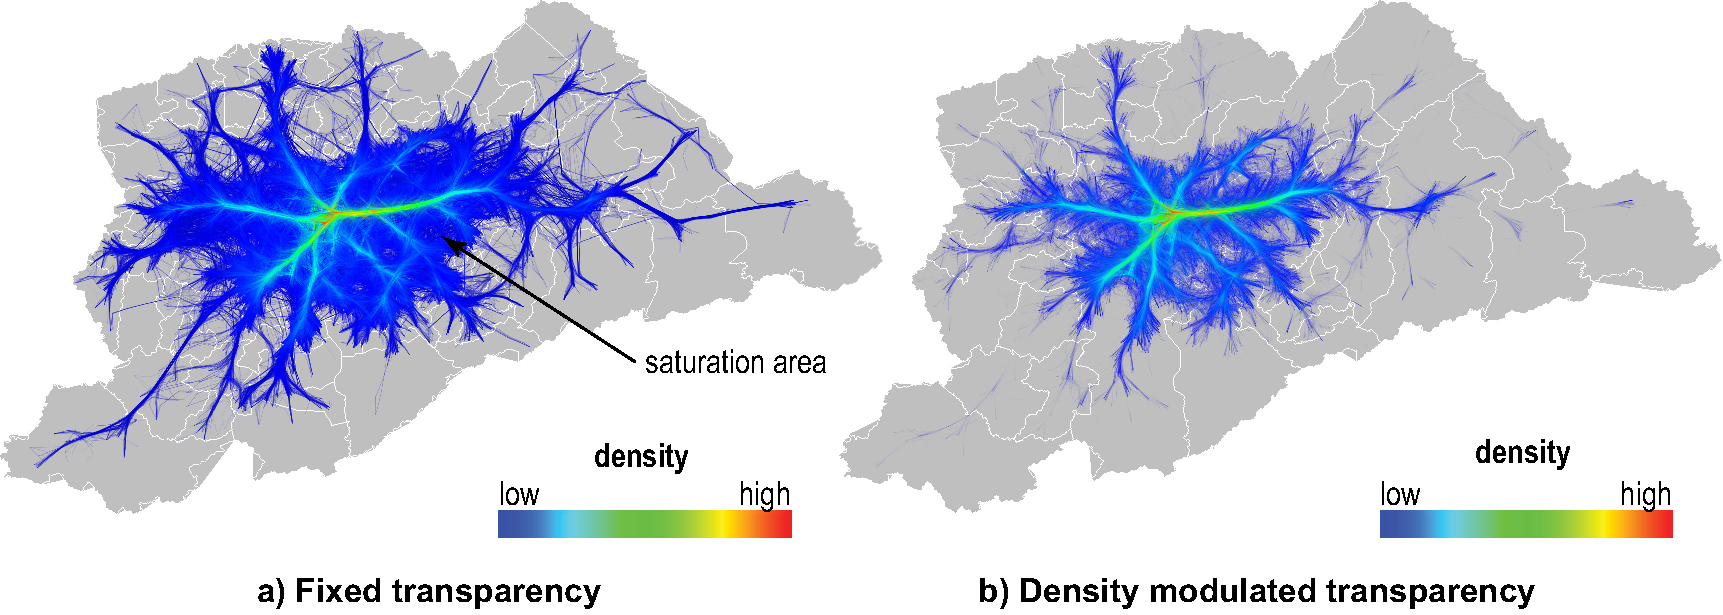
\includegraphics[width=0.98\textwidth]{../figuras/figure1}
  \caption{\emph{Bundling} das trajetórias coloridas pela densidade (a) valores fixos e \\(b) transparência modulada.}
  \label{fig:bundled-graph-density}  
\end{figure}

% % How we calculated 44%:
% %
% % 1. Take all trips that indicate bus, metro, and train as
% %    the main transportation mode -> this is the amount of
% %    trips by public transportation
% %
% % 2. Take all trips that indicate use of metro or train for
% %    some portion of the trip and divide that by the amount
% %    of trips by public transportation
% %
% % Using the tables from pages 46 and 49 of
% % http://www.metro.sp.gov.br/pesquisa-od/arquivos/Ebook%20Pesquisa%20OD%202017_final_240719_versao_4.pdf
% %
% % We consider that:
% % trips using bus as the main transportation mode: 8034
% % trips using train as the main transportation mode: 1245
% % trips using metro as the main transportation mode: 3400
% % total trips by public transportation: 8034 + 1245 + 3400 = 12679
% %
% % trips using metro for some portion of the trip: 3400
% % trips using train for some portion of the trip: 2272
% % total trips involving train or metro: 3400 + 2272 = 5672
% %
% % Percentage = 5672*100/12679 = 44.73%
% %
% % Not relevant for the text, just a curiosity:
% % the percentage in relation to all motorized trips is 5672*100/28280=20.05%

\section{Infraestrutura de metrô e trem \emph{vs} \emph{bundling}}
\label{sec:trail-overlap}

O sistema de transporte público é o mais utilizado pelos moradores da RMSP. O
impacto da malha ferroviária sobre o deslocamento de pessoas fica claro quando
desenhamos as linhas ferroviárias ao longo das trajetórias agrupadas com o
\emph{bundling}. A Figura~\ref{fig:rails} mostra a alta correspondência dos
\emph{bundles} com os caminhos das linhas ferroviárias (desenhadas em preto).
Tendo em vista que, de acordo com a pesquisa OD17, cerca de 44\% das viagens
diárias de transporte público envolvem metrô ou trens, este é um resultado
esperado. Curiosamente pode-se questionar se o sistema ferroviário foi planejado
com precisão para atender a demanda, como sugere a visualização agrupada, ou se
a disponibilidade dessa opção de transporte influenciou a existência de fluxos
tão densos. Embora não temos os insumos para responder a essa pergunta, os
gestores de tráfego podem usar esse tipo de visualização para elaborar políticas
para o transporte público. Apesar de não expressar nenhuma grande surpresa sobre os
dados analisados, este é um resultado bastante importante, pois consideramos que a alta
correlação entre o \emph{bundling} das trajetórias e as linhas das ferrovias
também indica boas configurações de parâmetros para esse tipo de visualização na
escala da região metropolitana.

Ressaltamos que que este tipo de correlação (de \emph{bundles} com estradas) não
é o mesmo que o utilizado no método RAEB, \cite{zeng:19}. No método RAEB, o
agrupamento foi feito explicitamente para seguir estradas. Em nosso caso, as
linhas são sobrepostas sobre \emph{bundles}, que foram gerados unicamente a partir dos
dados da OD. Pode-se argumentar que RAEB, neste sentido, produz \emph{bundles}
mais ``corretos'', uma vez que estes são forçados para seguir as estradas. No
entanto, olhando mais de perto, podemos ver que RAEB não pode ter todos os
\emph{bundles} seguindo precisamente todos os caminhos das estradas - pois isso
basicamente bloquearia qualquer agrupamento do \emph{bundling} e resultaria no próprio
mapa das estradas. Além disso, RAEB requer que o registro dos pontos das trajetórias
seja feito dentro de uma rede rodoviária precisa. Isso torna-o
significativamente mais complexo para implementar e mais caro para processar do
que nossa solução baseada em \emph{CUBu}.

\begin{figure}[!htb]
  \centering
  \captionsetup{justification=centering}
  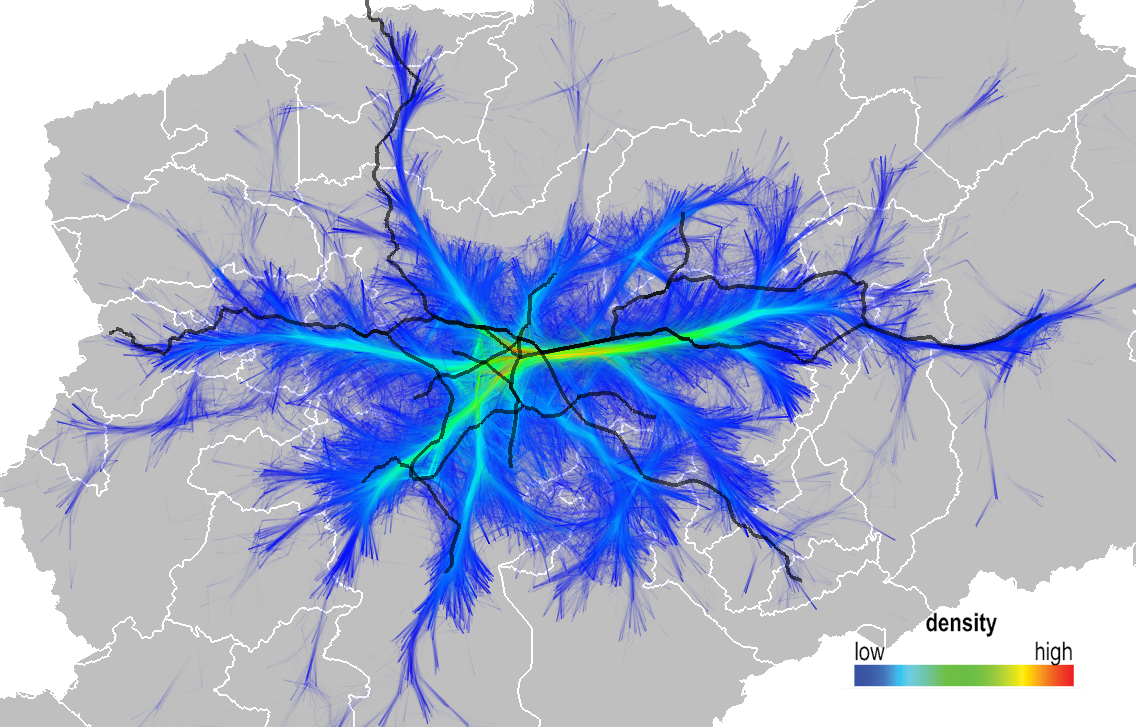
\includegraphics[width=0.98\textwidth]{../figuras/rail-lines.png}
    \caption{\emph{Bundling} das trajetórias coloridas pela densidade e a malha ferroviária da RMSP}
  \label{fig:rails}  
\end{figure}

\section{Mapeando distância e direção no \emph{bundling}}
\label{sec:length-direction}

Para explorar a mobilidade urbana de diferentes perspectivas, precisamos de
meios para visualizar seus múltiplos atributos de dados. No entanto, esta
variedade de atributos requer diferentes estratégias de visualização. Dois
importantes atributos para o estudo de padrões de mobilidade são distância
percorrida na viagem e a sua direção. As Figuras~\ref{fig:attributes-length} e
\ref{fig:attributes-direction} mostram a visualização de todo o conjunto de
dados OD17 mapeando a distância e direção, respectivamente.

A Figura~\ref{fig:attributes-length} exibe os comprimentos das viagens
codificados por cores. Nela utilizamos o mesmo mapa de cores arco-íris da
Figura~\ref{fig:rails} e também a modulação da transparência por densidade,
conforme explicado na Seção~\ref{sec:density}. Nesta imagem, podemos observar
uma única curva vermelha aparentemente na horizontal. Sua alta opacidade implica
que há muitas viagens longas, todas mapeadas perfeitamente para essa trajetória
entre a mesma origem e destino (se não o fizessem, veríamos um \emph{bundle} se
ramificando no formato de um leque em vez de uma curva precisa). Esta é uma
descoberta interessante que, argumentamos, não poderia ser facilmente encontrada
usando métodos não visuais. Apesar desse ponto incomum, as outras trajetórias,
em geral, percorrem distâncias regulares. \emph{Bundles} de longa distância como
este podem indicar falta de serviços ou recursos que não satisfazem as regiões
locais, obrigando as pessoas a percorrerem longas distâncias para acessá-los. A
pesquisa OD17 contém mais informações que podem ajudar a investigar o motivo
dessas longas viagens.

A Figura~\ref{fig:attributes-direction} mostra os mesmos dados da
Figura~\ref{fig:attributes-length}, mas ao invés da distância são as direções
das viagens que estão codificadas em cores. Para este atributo em específico,
usamos ainda um recurso do \emph{CUBu}, que separa trilhas em direções opostas
em dois \emph{bundles} quase paralelos. Podemos ver claramente a existência de
trajetórias paralelas ao longo dos \emph{bundles}, o que não é surpreendente
porque a pesquisa OD registra o trajeto típico das pessoas que inclui os
deslocamentos de ida e vinda de volta para suas origens. No entanto, essa
simetria das trajetórias possivelmente não seria observada se analisássemos um
curto período do dia.

\begin{figure}[!htb] \centering \captionsetup{justification=centering}
  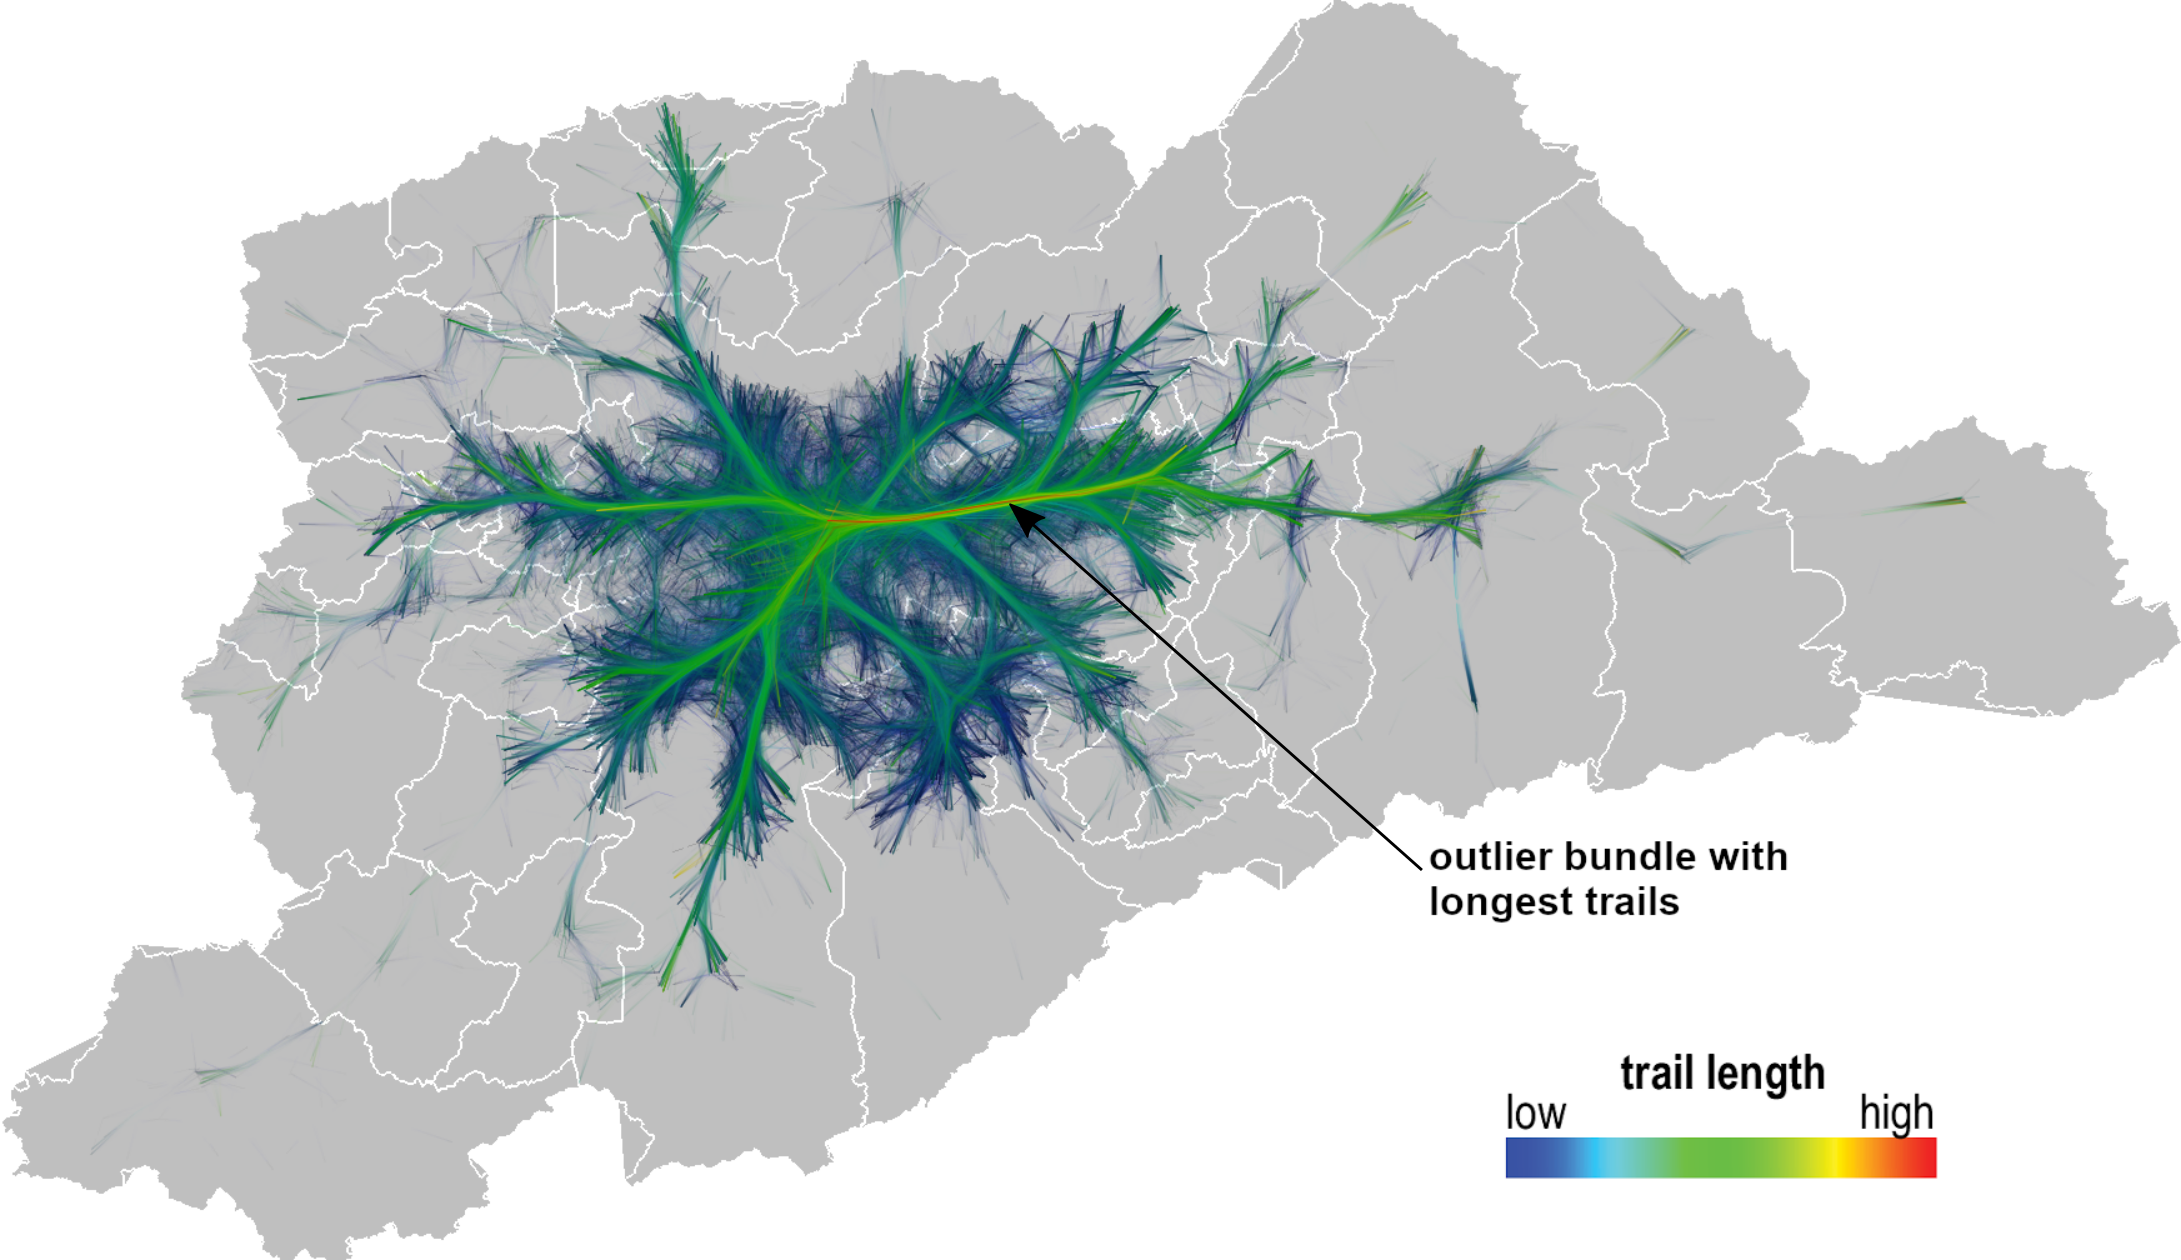
\includegraphics[width=0.98\textwidth]{../figuras/distances.png}
  \caption{Mapeamento da distância das viagens em cores. \label{fig:attributes-length}}
  \end{figure}

\begin{figure}[!htb]
  \centering
  \captionsetup{justification=centering}
  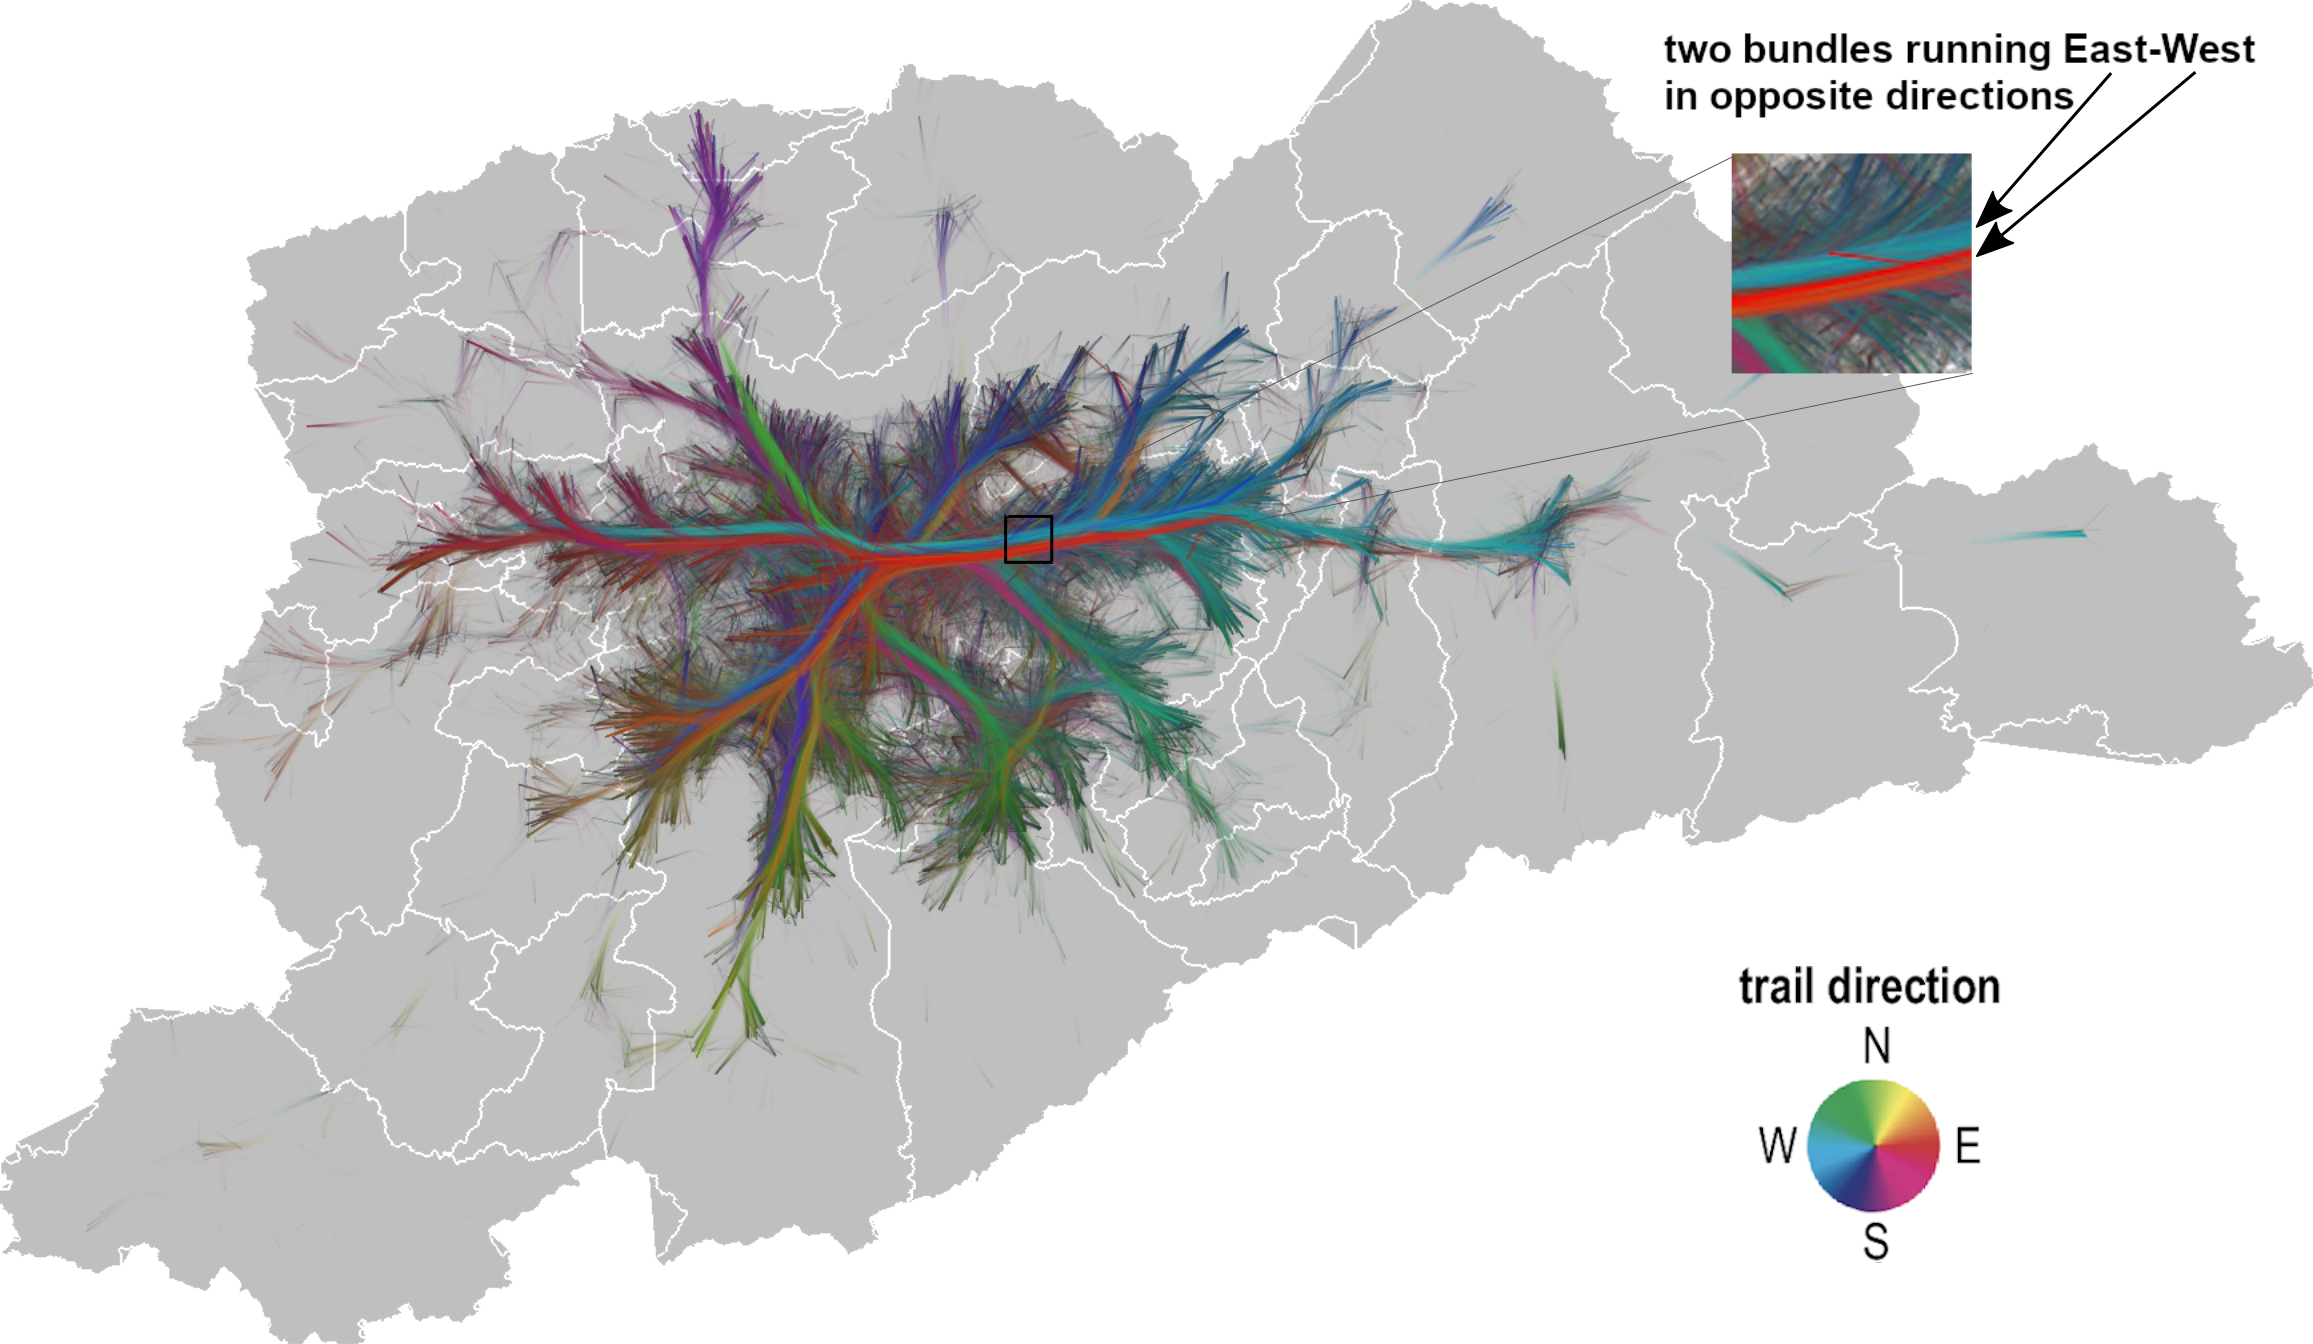
\includegraphics[width=0.98\textwidth]{../figuras/directions.png}
  \caption{Mapeamento da direção das viagens em cores. \label{fig:attributes-direction}}
\end{figure}

\section{Coloring transportation modes: local \emph{vs} intercity buses}
\label{sec:coloring}
% %
% The OD17 dataset contains 17 transportation modes. While it would be ideal to be able to see the 17 categories all at once in our bundled visualization, that would not be easy to do, since it would require the simultaneous encoding of 17 different categorical attributes. Instead, we use transparency to hide trails according to a user-set selector that filters them by transportation mode. Figure~\ref{fig:bus-integration} shows how we can use these filters to visualize the integration between buses from the city of S\~ao Paulo (local buses) and intercity buses. %Unbundled and bundled trajectories are presented on the left and right sides respectively.
% Each transportation mode has a distinct color -- olive for local buses and blue for intercity buses.

% Figure~\ref{fig:bus-integration} also highlights that these different transportation systems appear to complement each other. The city of S\~ao Paulo has a very active commerce and industry, and many people from neighboring cities work there. Thus, the availability of public transportation and its integration is very important for these people. This kind of filtering along with bundling helps to better understand correlations between data attributes -- in this case, \hbox{transportation}~modes.


% \begin{figure}[!htb]
%   \centering
%   \captionsetup{justification=centering}
%   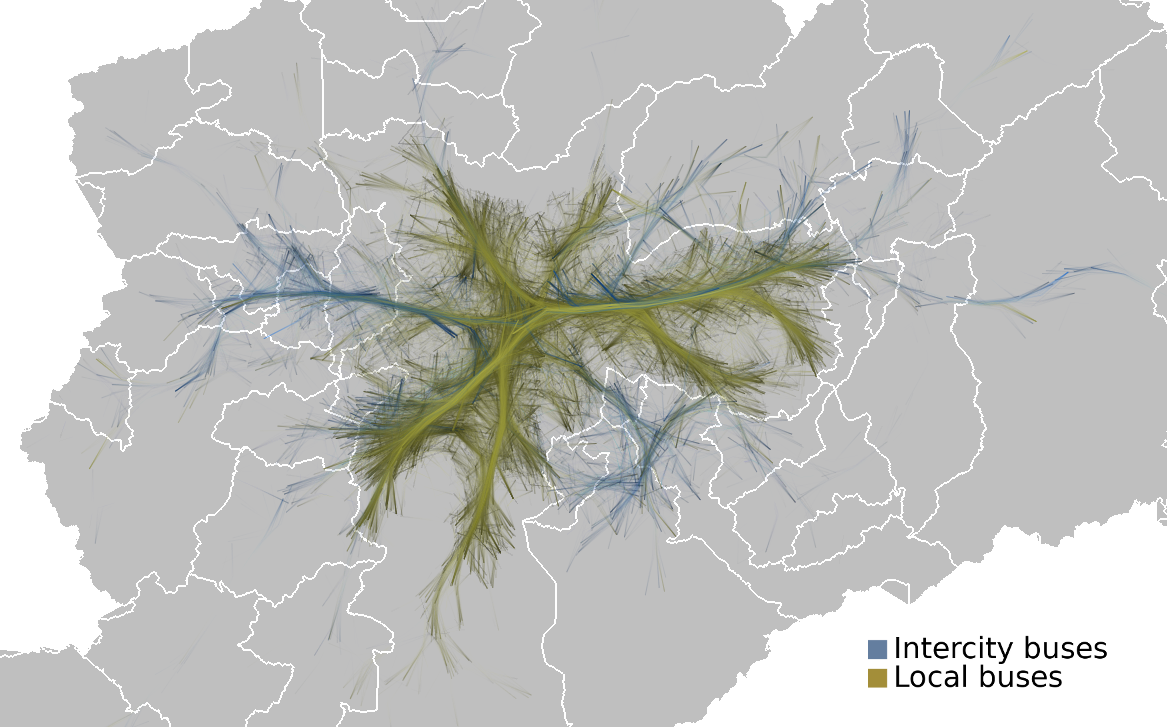
\includegraphics[width=0.98\textwidth]{figures/local-intercity-buses}
%   \caption{Edges filtered by transportation modes: bundled trails of local and intercity buses. \label{fig:bus-integration}}
% \end{figure}

\section{Density per social strata}
\label{sec:strata}
% % 6 imagens, uma de cada classe social, density1
% We used our bundle visualization to study how citizens with different economical conditions commute in the SPMA. The Brazilian Economical Classification Criterion (BECC)\,\cite{cceb2008} is the official social-economic index used in the Brazilian Demographic Census, which is performed by the Brazilian Institute of Geography and Statistics. It measures the purchasing power of the Brazilian society. The BECC is divided into six levels or strata (Table~\ref{tab:becc}). This index is used in the OD17 survey to complement the mobility data. Table~\ref{tab:becc} also shows the average monthly income in the local currency (Brazilian reals) and in US dollars, and the number of trips in the SPMA for each BECC level considering the whole population and only citizens with age between 6 and 18 years that commute for study (see Section~\ref{sec:students}).

% To compare the mobility patterns of different BECC social strata, we bundled the trails in each stratum separately, as shown in Figures~\ref{fig:becc-axd-e}~to~\ref{fig:becc-d-e}. We see significant differences in the mobility patterns between the highest and lowest income levels as shown in Figure~\ref{fig:becc-axd-e}. The $A$ level (on the left-hand side) has a high density in the center of SPMA, which includes the capital downtown surroundings. The highest density is located in the west, southwest, and northeast neighborhoods near downtown. There are density flows between the capital and the cities of Barueri and Cotia, which have high-income residential areas. There are other high dense flows linking the capital to the cities of S\~ao Bernardo do Campo and Santo Andr\'e. Comparing $A$ to the $D$-$E$ level (on the right-hand side of Figure~\ref{fig:becc-axd-e}), we see that $D$-$E$ has the highest dense flows in the capital eastern region. In the $D$-$E$ level map, we can see the absence of high-dense flows in regions that are nearest to the capital downtown; in contrast, these are present in the $A$ level map. We can see more details of $A$ and $D$-$E$ strata in Figures~\ref{fig:becc-a}~and~\ref{fig:becc-d-e}

% \begin{figure}[!htb]
%   \centering
%   \captionsetup{justification=centering}
%   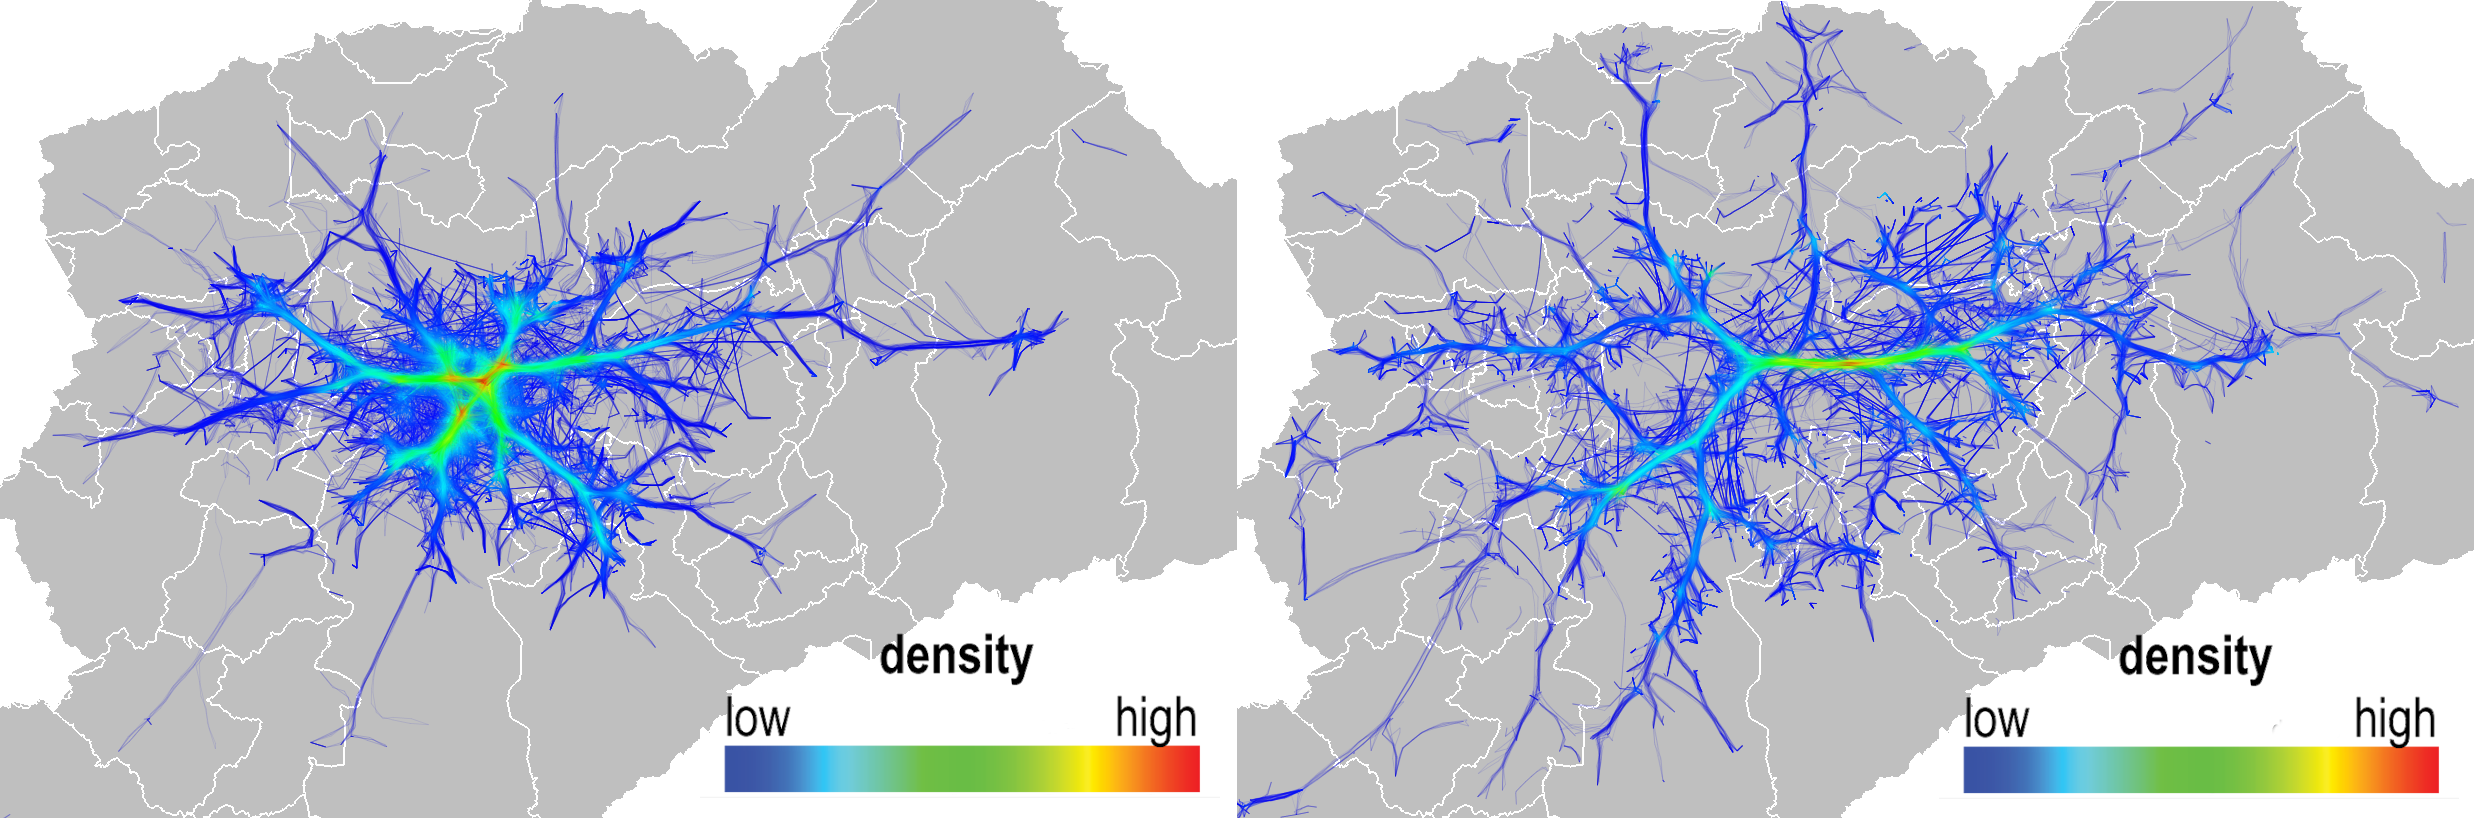
\includegraphics[width=0.98\textwidth]{figures/comparison-axd-e-strata-leg.png}
%   \caption{Comparing density of trails between social strata $A$ (left-hand side) and $D$-$E$ (right-hand side). \label{fig:becc-axd-e}}
% \end{figure}


% \begin{figure}[!htb]
%   \centering
%   \captionsetup{justification=centering}
%   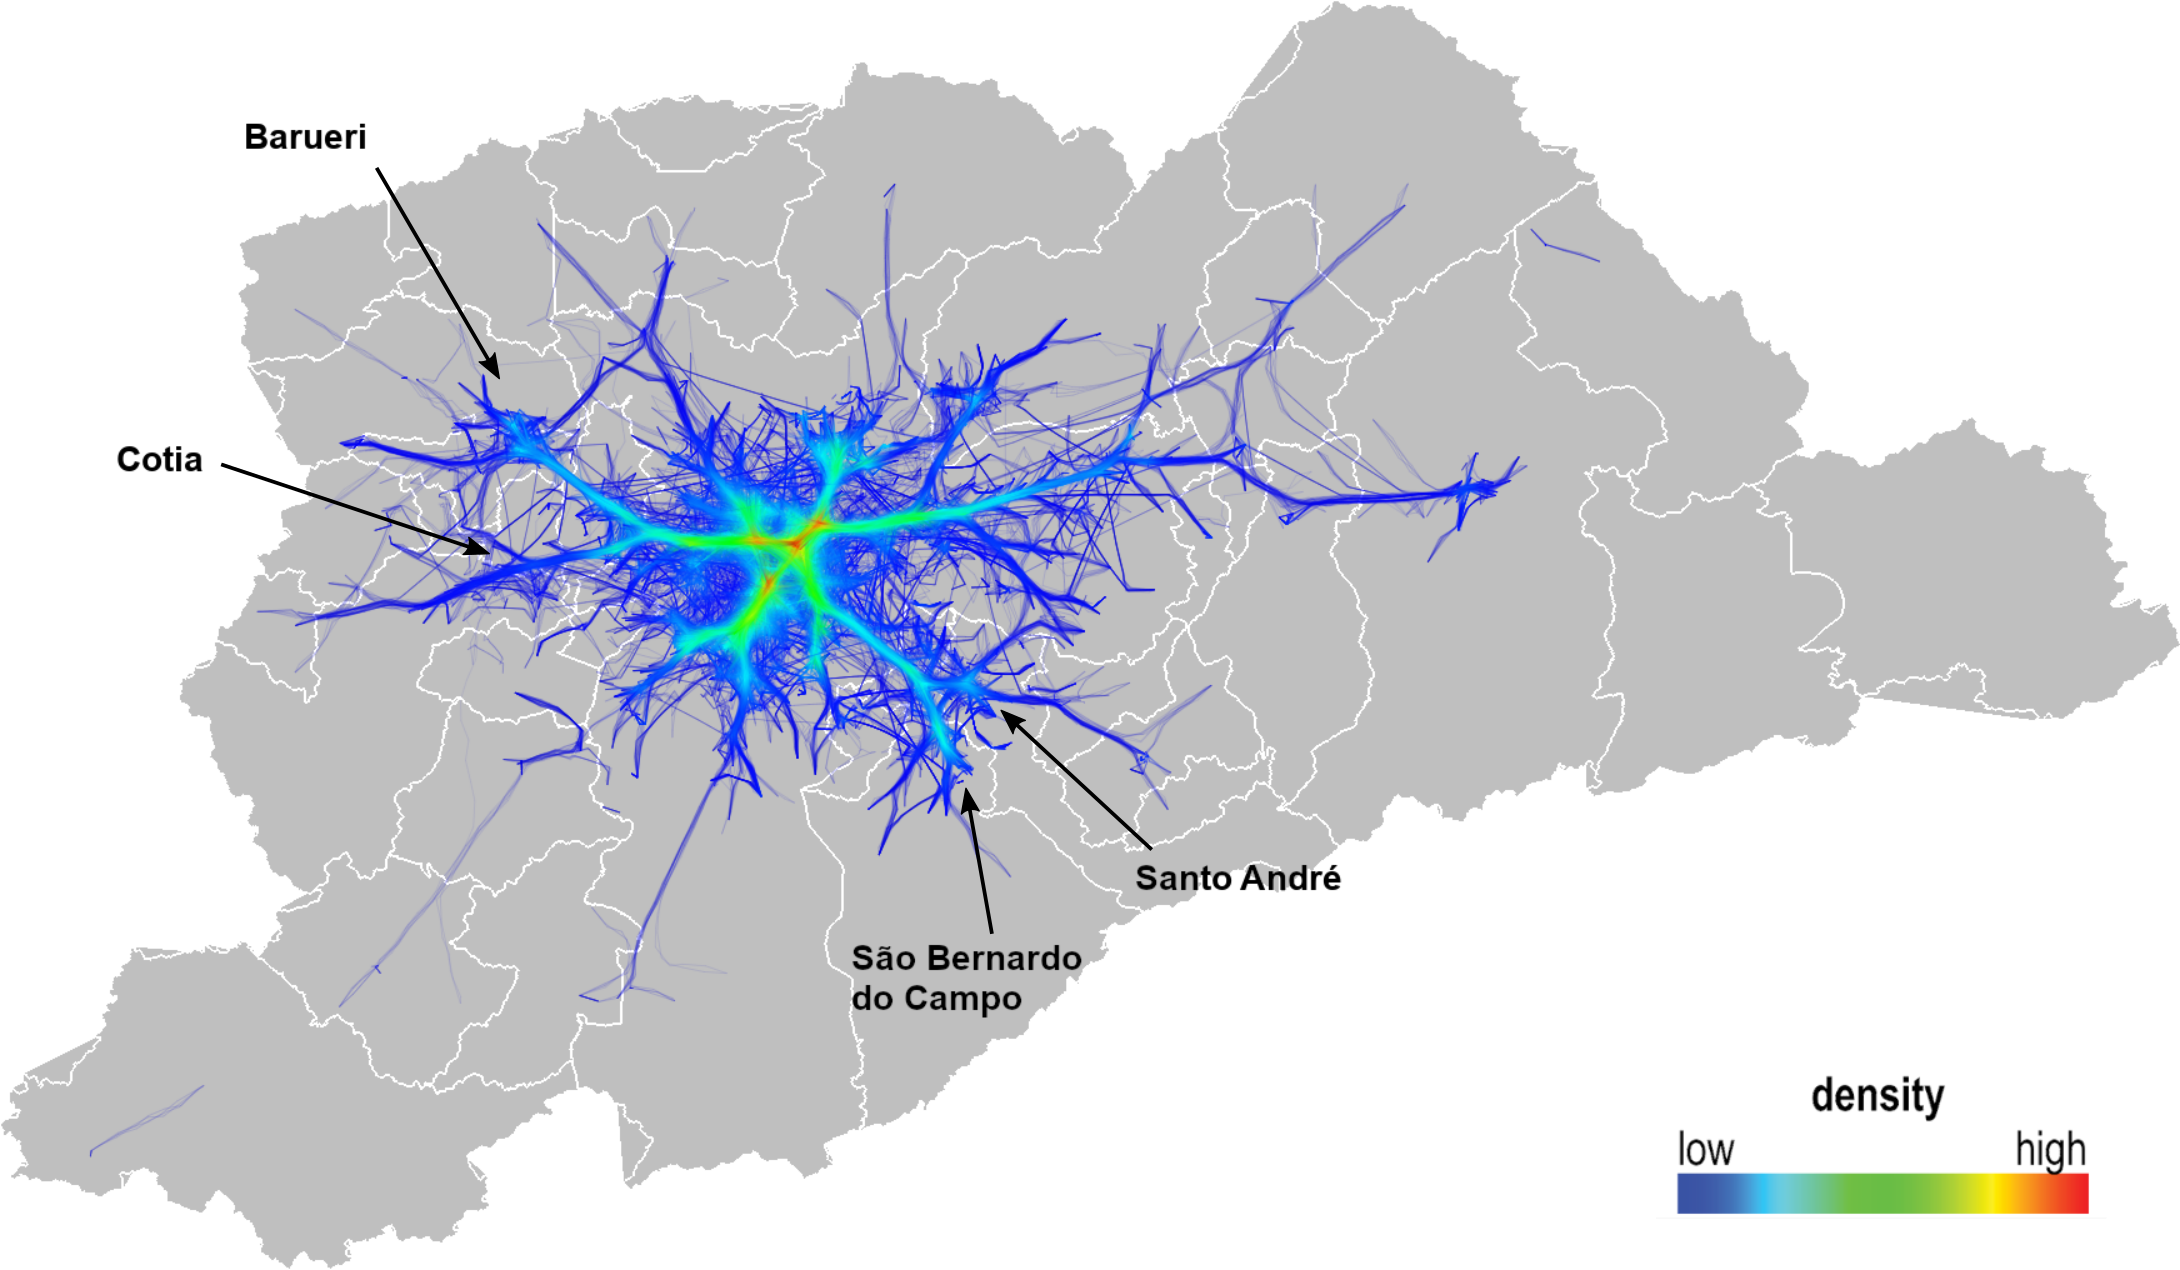
\includegraphics[width=0.98\textwidth]{figures/1-class-a.png}
%   \caption{Density of trails of social stratum $A$. \label{fig:becc-a}}
% \end{figure}

% \begin{figure}[!htb]
%   \centering
%   \captionsetup{justification=centering}
%   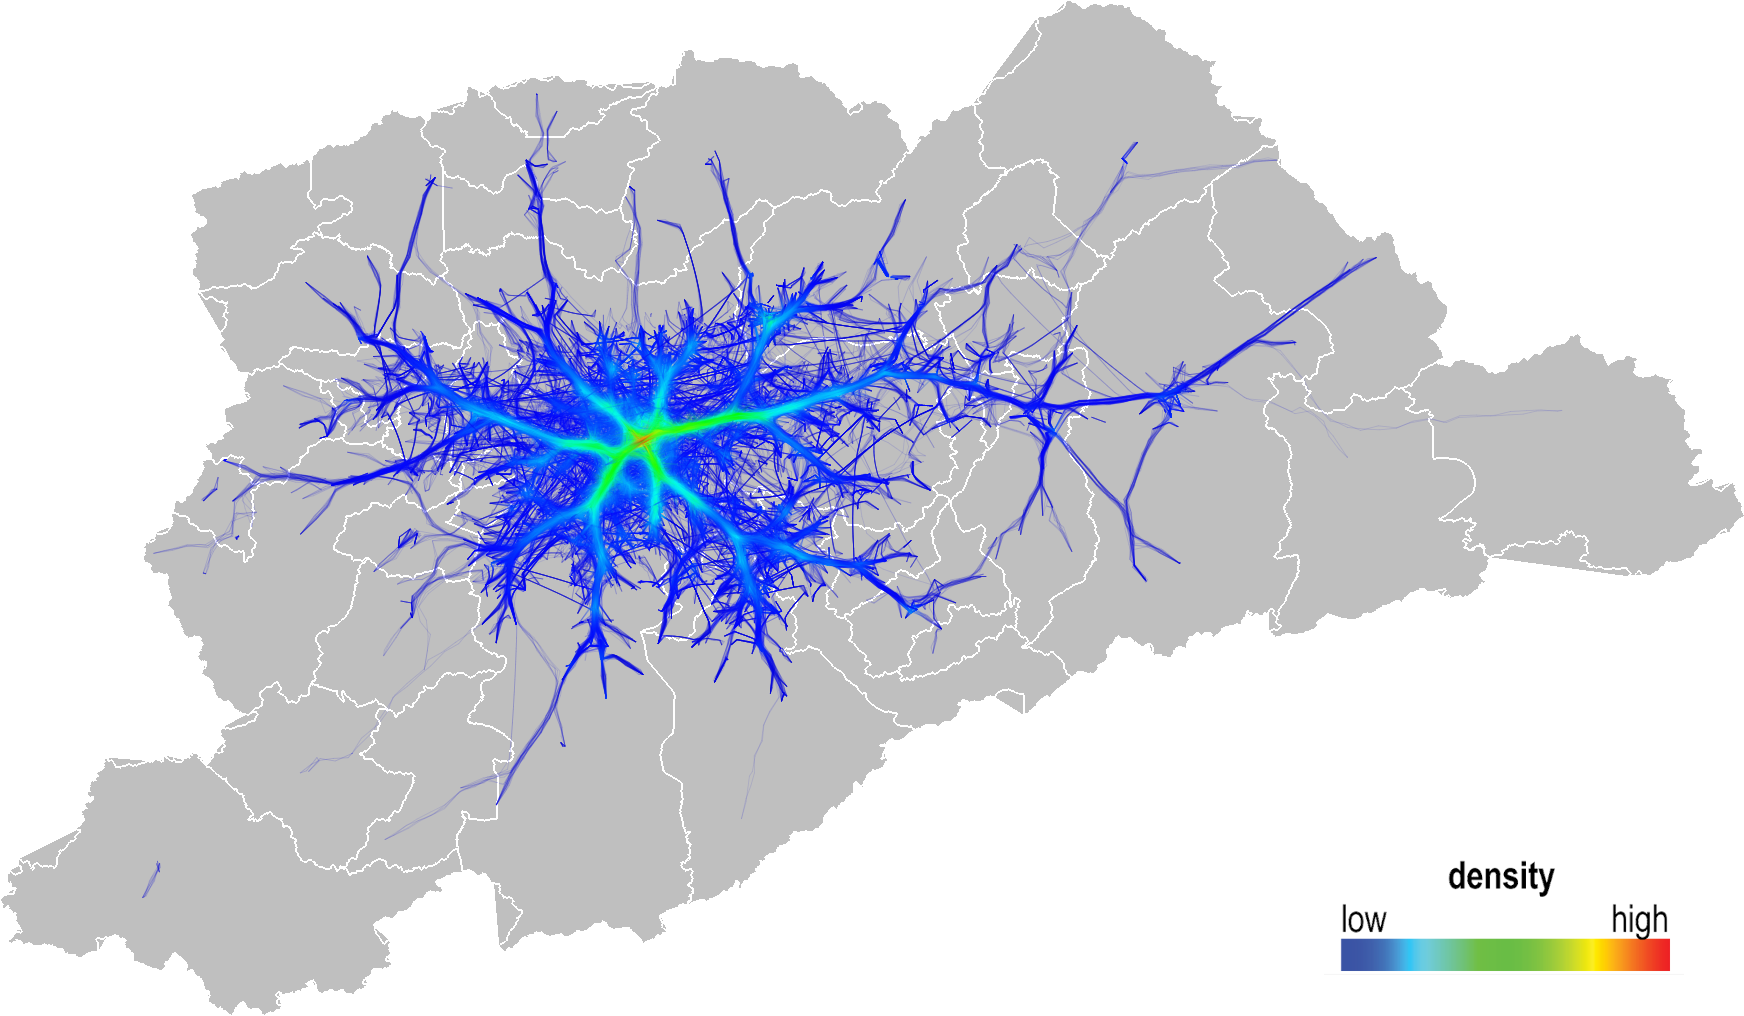
\includegraphics[width=0.98\textwidth]{figures/2-class-b1.png}
%   \caption{Density of trails of social stratum $B1$. \label{fig:becc-b1}}
% \end{figure}

% \begin{figure}[!htb]
%   \centering
%   \captionsetup{justification=centering}
%   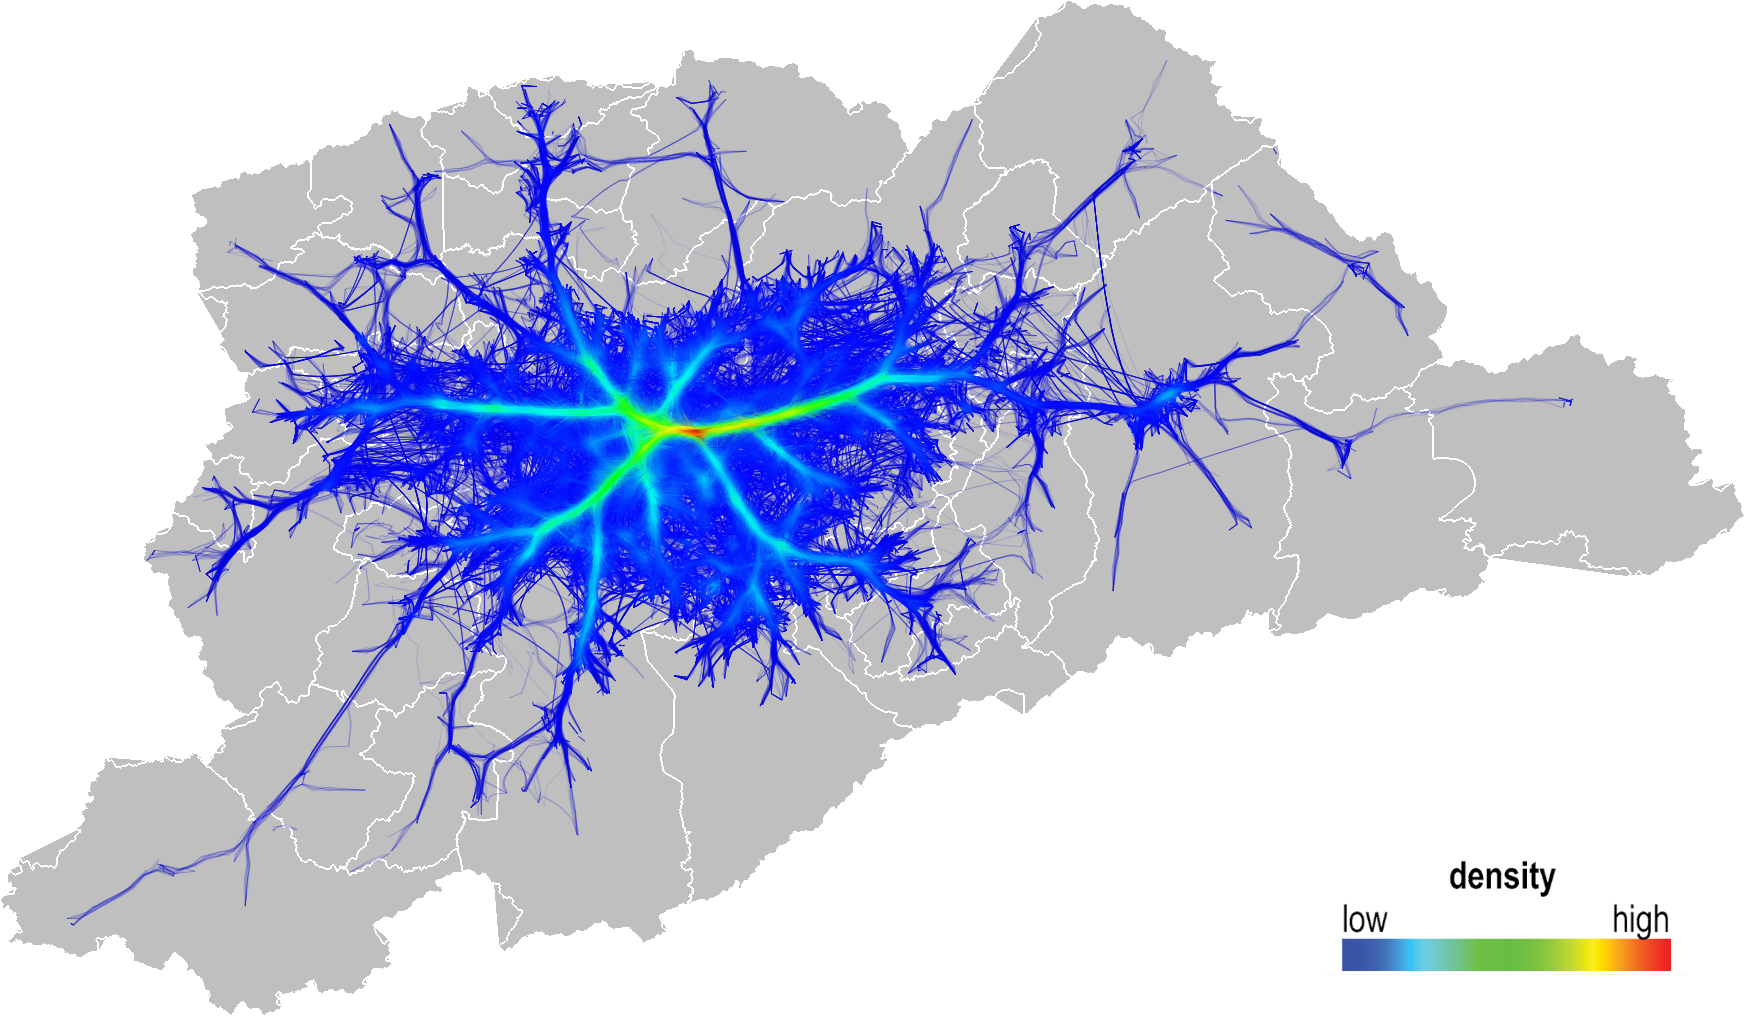
\includegraphics[width=0.98\textwidth]{figures/3-class-b2.png}
%   \caption{Density of trails of social stratum $B2$. \label{fig:becc-b2}}
% \end{figure}

% \begin{figure}[!htb]
%   \centering
%   \captionsetup{justification=centering}
%   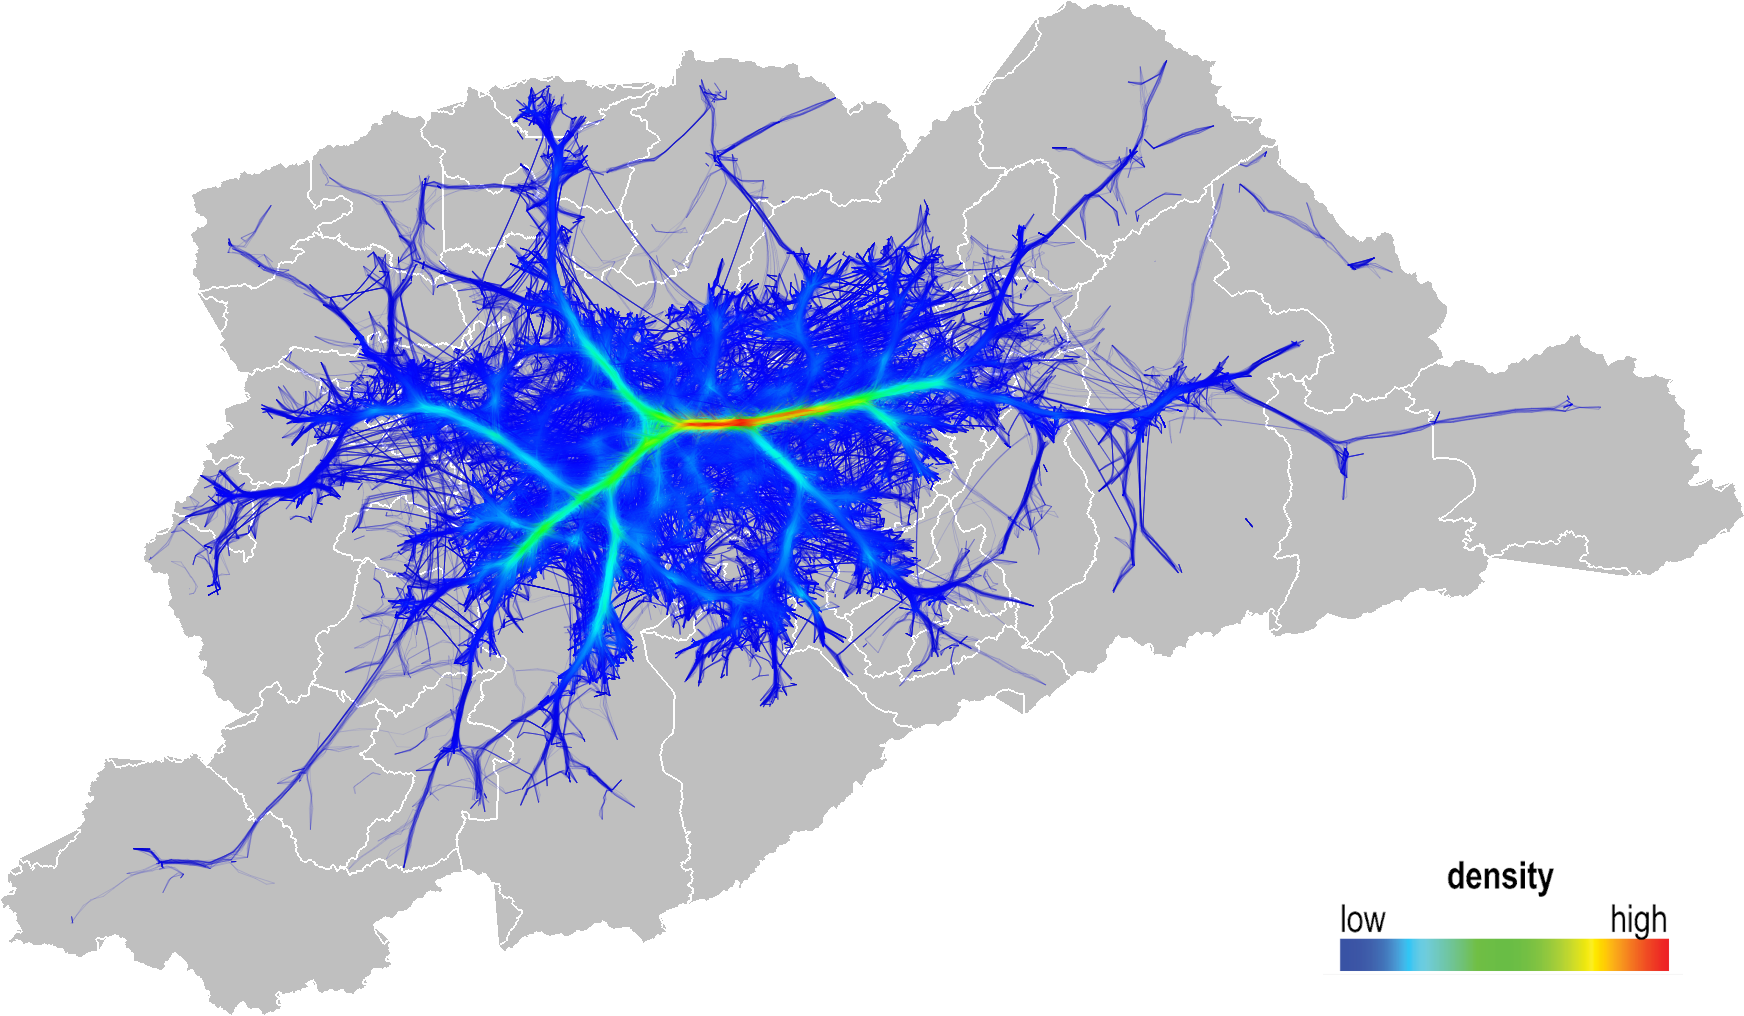
\includegraphics[width=0.98\textwidth]{figures/4-class-c1.png}
%   \caption{Density of trails of social stratum $C1$. \label{fig:becc-c1}}
% \end{figure}

% \begin{figure}[!htb]
%   \centering
%   \captionsetup{justification=centering}
%   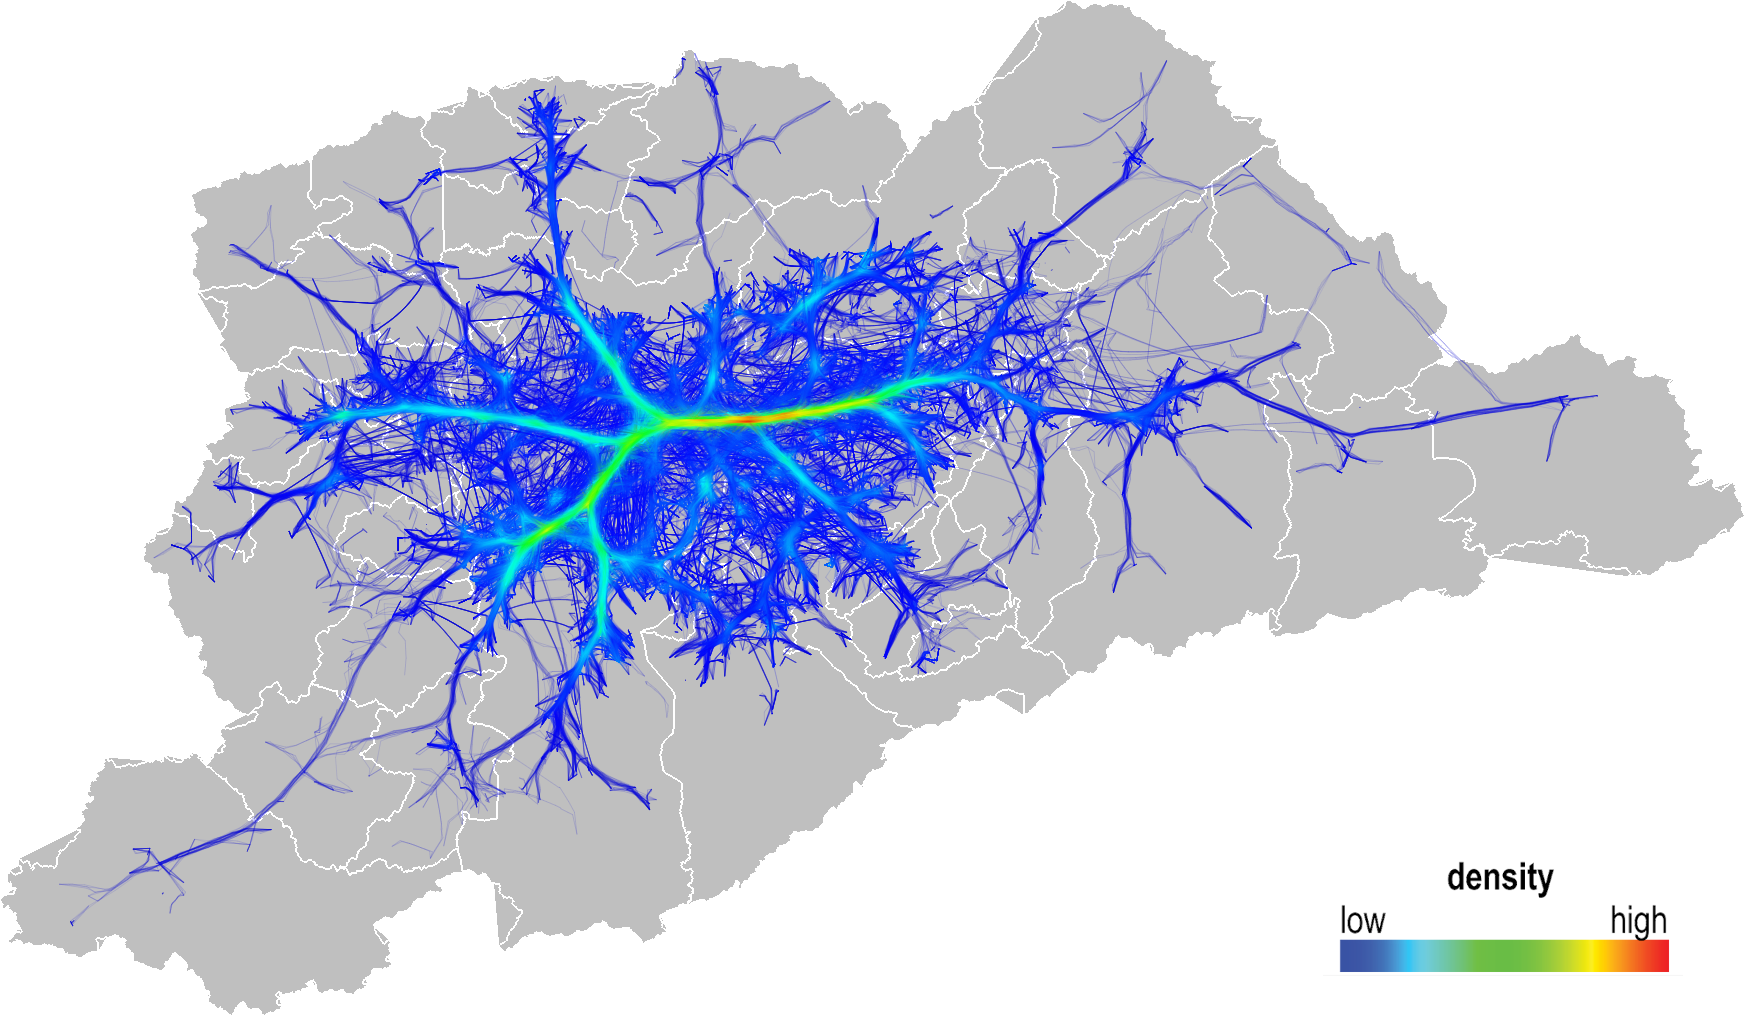
\includegraphics[width=0.98\textwidth]{figures/5-class-c2.png}
%   \caption{Density of trails of social stratum $C2$. \label{fig:becc-c2}}
% \end{figure}

% \begin{figure}[!htb]
%   \centering
%   \captionsetup{justification=centering}
%   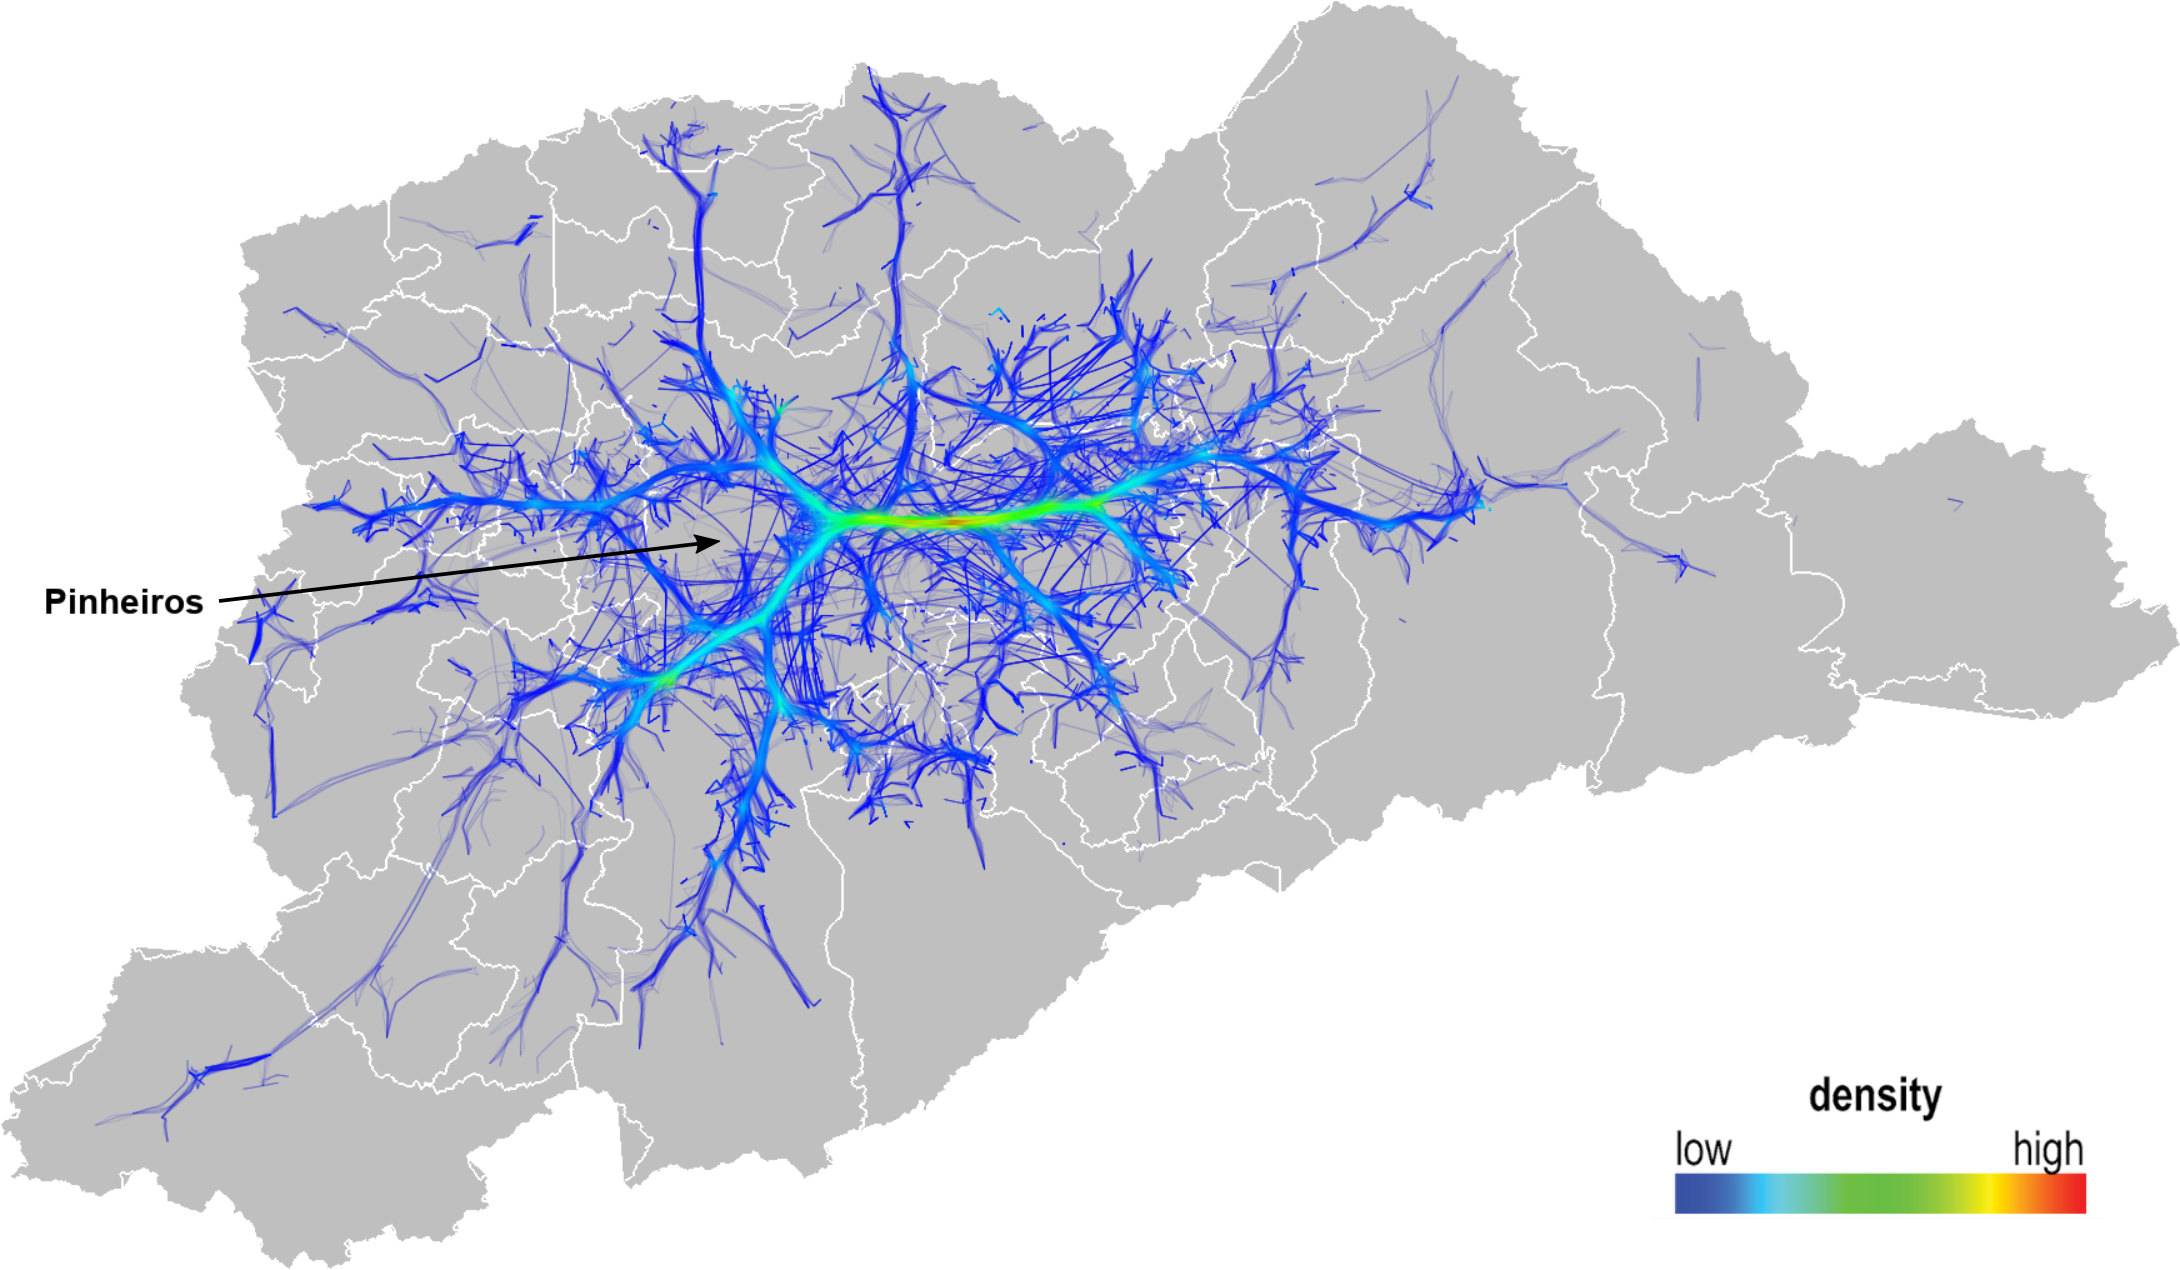
\includegraphics[width=0.98\textwidth]{figures/6-class-d-e.png}
%   \caption{Density of trails of social strata $D$-$E$. \label{fig:becc-d-e}}
% \end{figure}

% When we compare all maps from the $A$ to the $D$-$E$ level (Figures~\ref{fig:becc-a}~to~\ref{fig:becc-d-e}), we see that the densest flows (red) tend to displace from the capital downtown to the eastern region of the city. The concentration of high-density flows is increasingly spreading from the center to the peripheral regions of the SPMA. Even the less dense flows are increasing and spreading over the SPMA. However, the $D$-$E$ map shows that those flows diminish considerably for these social strata. This may indicate that low-income citizens have less access to the urban mobility system. As a consequence, these people would have less access to the social, educational, health, and cultural services of the SPMA, as those facilities are concentrated in the center regions of the cities. It is worthy to note that those central regions also have more job opportunities. Looking at the $D$-$E$ map, we can see a ``hole" in the capital west downtown. This region (Pinheiros district) concentrates a large number of jobs related to information technology and financial services, which requires workers with high and medium education levels. Thus, the map shows that low-income citizens are not going to that region, which reflects the inequality of opportunities that these citizens face.

% \begin{table}[!htb]
%   \small
%   \newcommand{\hdr}[1]{\bfseries#1}
%   \centering
%   \caption{Trips grouped per BECC income level, social stratum, and traveler age.\label{tab:becc}}
%   \begin{tabular}{>{\footnotesize}c>{\footnotesize}r>{\footnotesize}r>{\footnotesize}r>{\footnotesize}r}
%     \toprule
%     \multirow{2}[2]{*}{\hdr{BECC level}} & \hdr{Monthly income} & \hdr{Monthly income}& \multirow{2}[2]{*}{\hdr{Trips}} & \hdr{Trips of 6 to 18}\\
%     & \hdr{(Brazilian reals (R\$))} & \hdr{(US dollars ($\sim$US\$))} & & \hdr{years old students}\\
%     \midrule
%     A   & 23,345    & 4,245 & 3,062,892  &   184,772\\
%     B1  & 10,386    & 1,888 & 3,854,040  &   260,652\\
%     B2  & 5,363     & 975   & 12,856,182 &   963,242\\
%     C1  & 2,965     & 539   & 11,277,159 &   976,745\\
%     C2  & 1,691     & 307   & 7,852,806  &   721,218\\
%     D-E & 708       & 128   & 2,233,801  &   219,612\\
%     \bottomrule
%   \end{tabular}
% \end{table}

\section{Mobility of young students from different social strata}
\label{sec:students}
% % od17-escola-alta-renda-6-18, od17-escola-baixa-renda-6-18 density1
% To explore even more the mobility patterns showed bundling visualizations, we compared the trips of students from different social strata. We filtered citizens with age between 6 and 18 years whose commuting reason is study. We split them into two groups, the high- to moderate-income, which includes the BECC levels $A$, $B1$, $B2$, and $C1$; and the low-income, which includes levels $C2$ and $D$-$E$. Figures~\ref{fig:students-high}~and~\ref{fig:students-low} show the density maps for both groups.

% \begin{figure}[!htb]
%   \centering
%   \captionsetup{justification=centering}
%   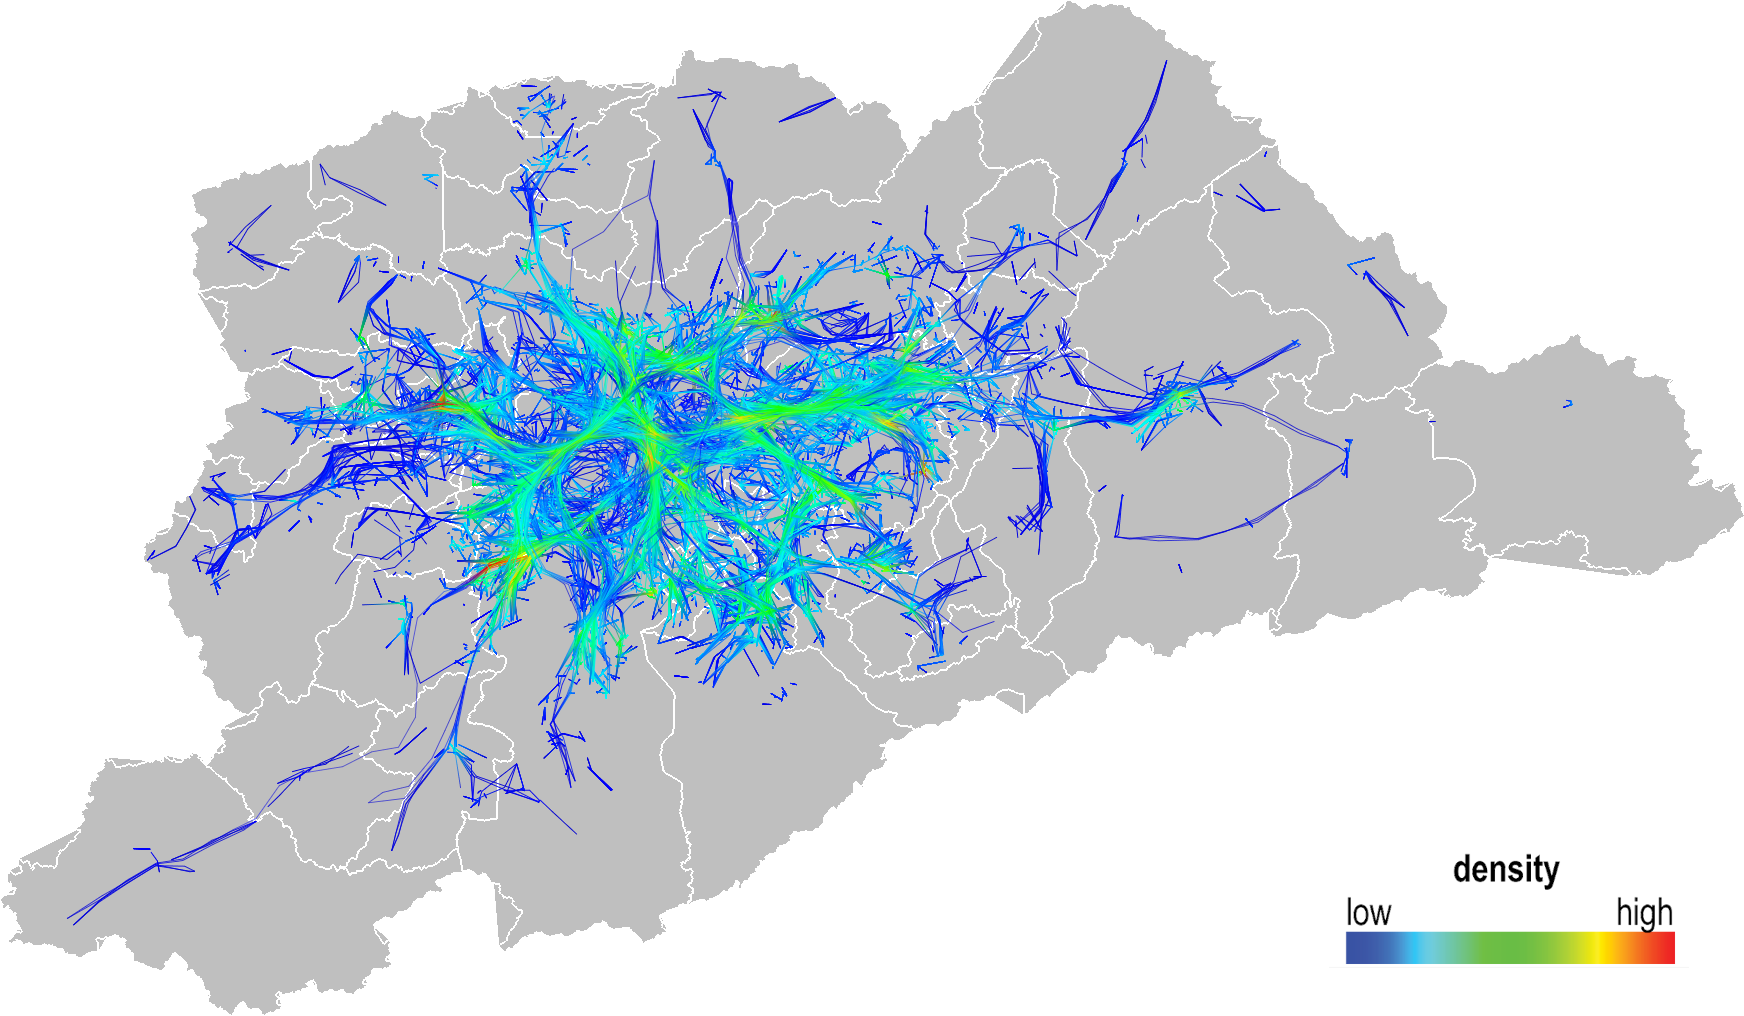
\includegraphics[width=0.98\textwidth]{figures/high-income-density-leg.png}
%   \caption{Density of trails of young students from high-income households. \label{fig:students-high}}
% %\end{figure}
% \vspace*{\floatsep}
% %\begin{figure}[!htb]
%   \centering
%   \captionsetup{justification=centering}
%   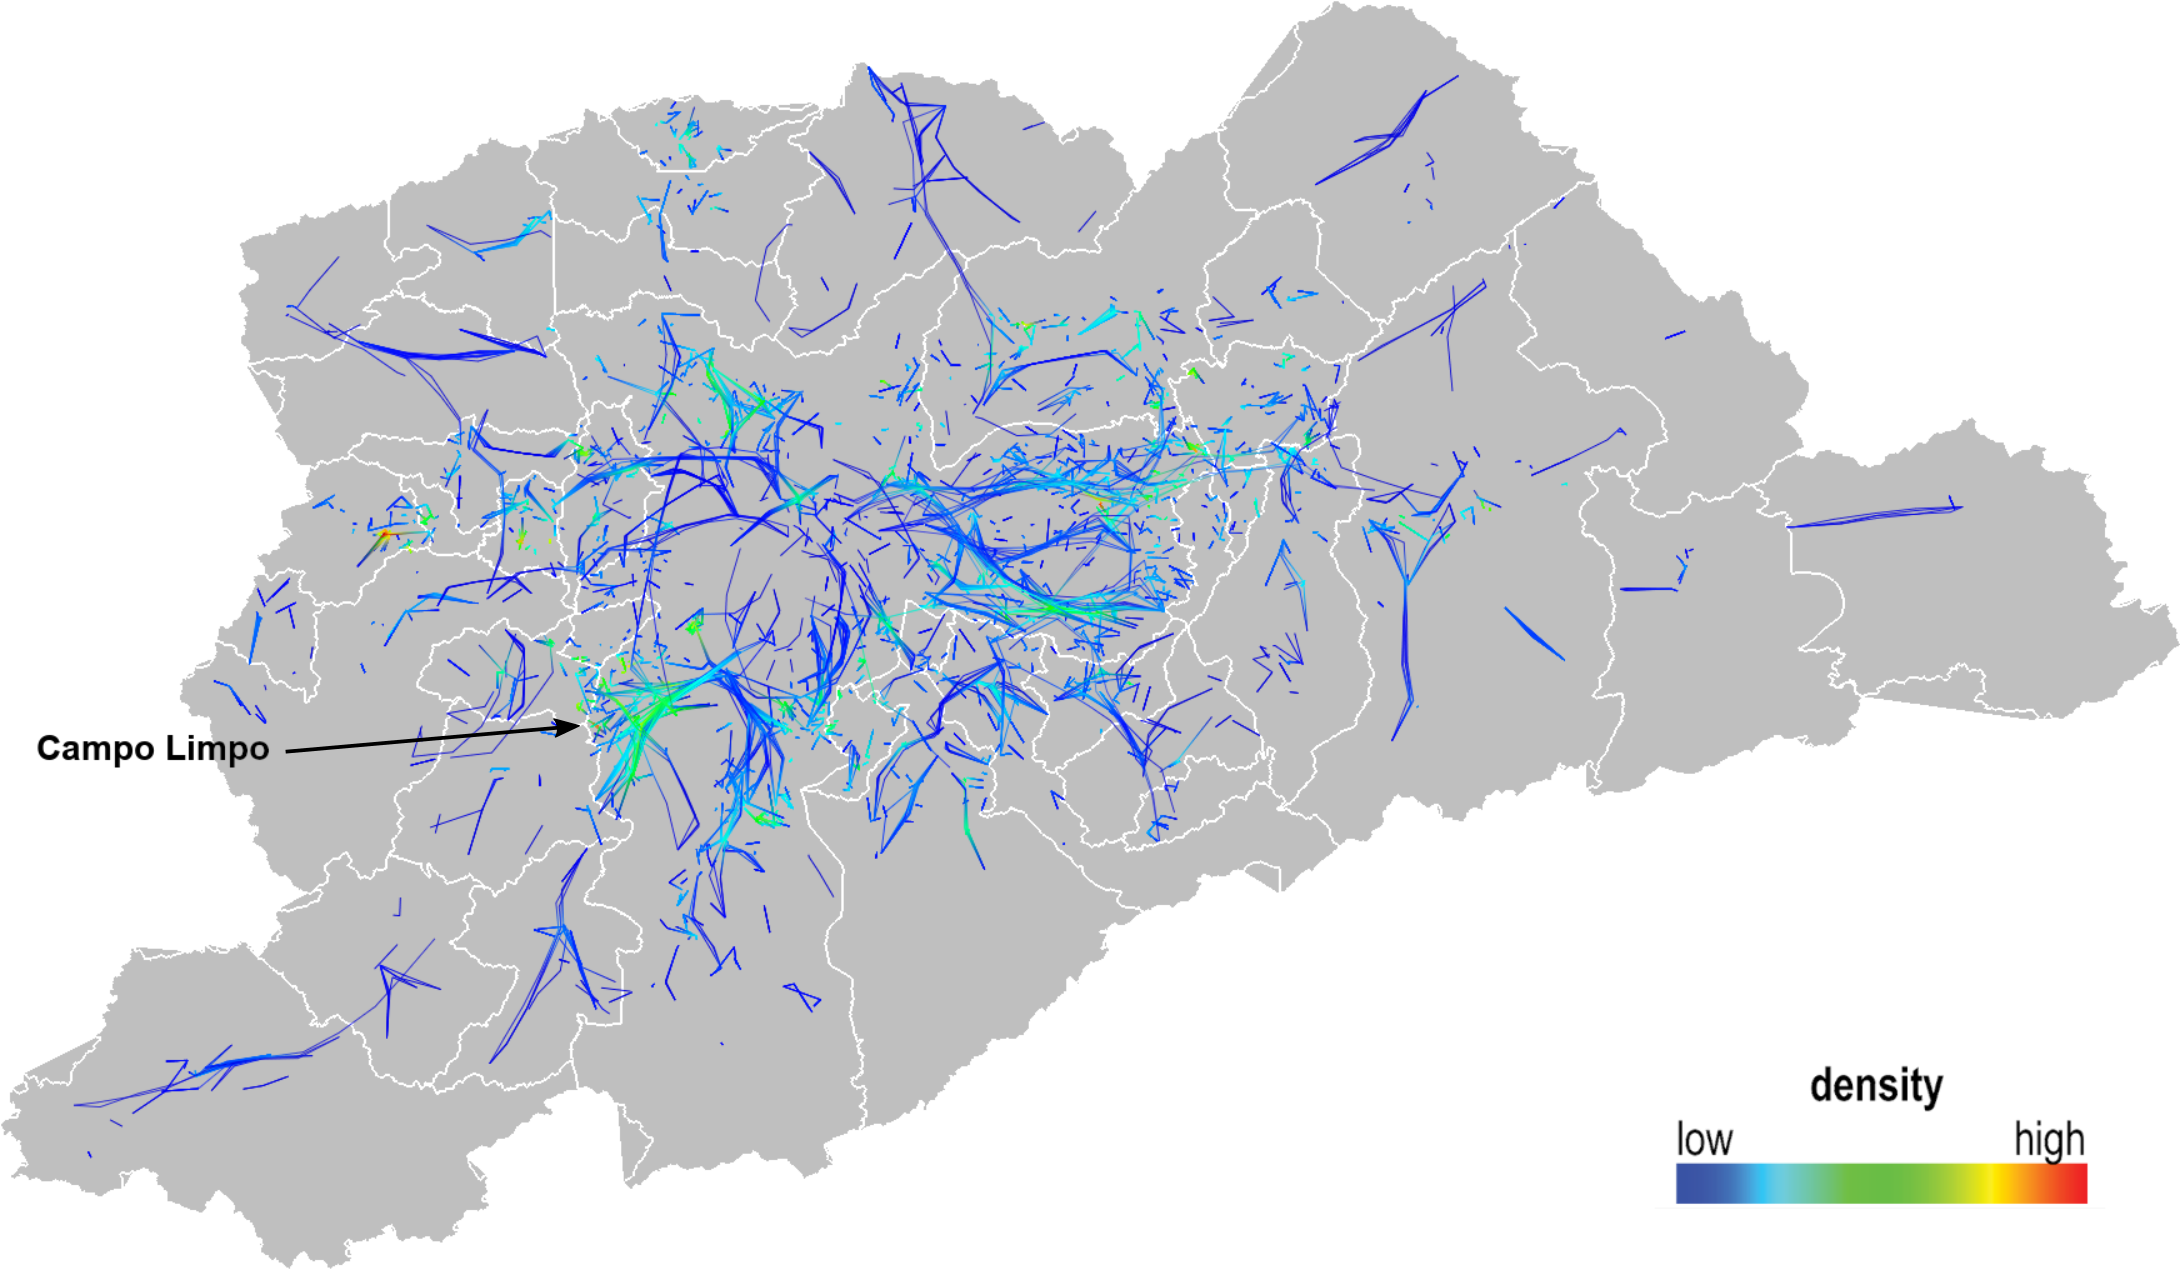
\includegraphics[width=0.98\textwidth]{figures/low-income-density-leg.png}
%   \caption{Density of trails of young students from low-income households. \label{fig:students-low}}
% \end{figure}

% The density map of the high- to moderate-income students (Figure~\ref{fig:students-high}) shows a large number of dense flows spread across the central region of SPMA. This part of SPMA concentrates most private schools, universities, and complementary colleges. In addition, high density flows are not as long as flows from other maps with all the data (e.g., Figure~\ref{fig:bundled-graph-density}). This indicates that trips to study are shorter than trips to work. 

% The density map of low-income students (Figure~\ref{fig:students-low}) shows that their mobility is very limited compared to the higher-income students. There are a few dense flows, most of them out of the capital downtown. The high density flows of low-income students are more present in the peripherals of the capital and also in the neighboring cities. There is a concentration of both groups in the southwest region, where are the neighborhoods of the Campo Limpo district. 

% It is worthy to note that the public schools in the SPMA are spread across the central and peripheral parts of the cities. The students are enrolled in these schools according to the proximity of their residences. Thus, they do not have to travel long distances to reach their schools. Also, public schools have lower educational performance than private schools in S\~ao Paulo. Thus, citizens with better financial conditions use to put their children in private schools.

% The scarcity of flows from low-income students may indicate that they do not have equal opportunities to study, being enrolled in schools in their neighborhood. They also do not use to go to the central region of the city and, thus, have less access to universities and complementary colleges. This inequality of opportunities will probably impact these students' jobs and economical conditions.

% We also see that there are many more trails for the high- to moderate-income students (Figure~\ref{fig:students-high}) than for low-income students (Figure~\ref{fig:students-low}). The high-to moderate-income students also travel large distances to study, which indicates that they can choose more flexibly where to study. This fact is corroborated by urban mobility studies that indicate that people with better financial conditions have more mobility than those with poorest conditions\,\cite{carruthers2005,lucas2016}.

\section{Directions at peak hours}
\label{sec:peak-hours}
% %
% As discussed earlier in Sec.~\ref{sec:data}, Figure~\ref{fig:trips_by_hour} shows the distribution of trips by hour of the day, with two main rush-hour peaks (6-9 AM and 5-8 PM). 
% However, this aggregated table does not give us insights in how the rush-hour patterns may differ. To see this, we selected the two rush-hour time intervals and visualized them separately, using directional bundling and color-coding.

% \begin{figure}[!htb]
%   \centering
%   \captionsetup{justification=centering}
%   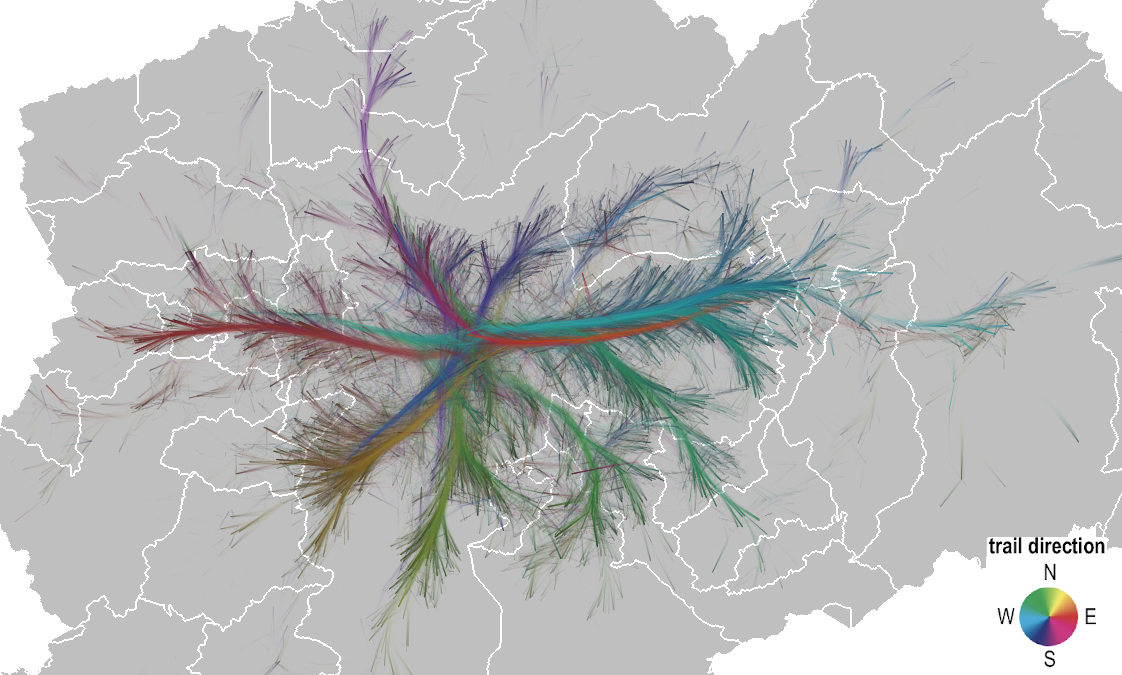
\includegraphics[width=0.98\textwidth]{figures/peak-hours-6h-to-9h-direction-leg.png}
%   \caption{Directions of trips between 6 to 9 AM \label{fig:peak-hours-6h-9h}}
% %\end{figure}
% \vspace*{\floatsep}
% %\begin{figure}[!htb]
%   \centering
%   \captionsetup{justification=centering}
%   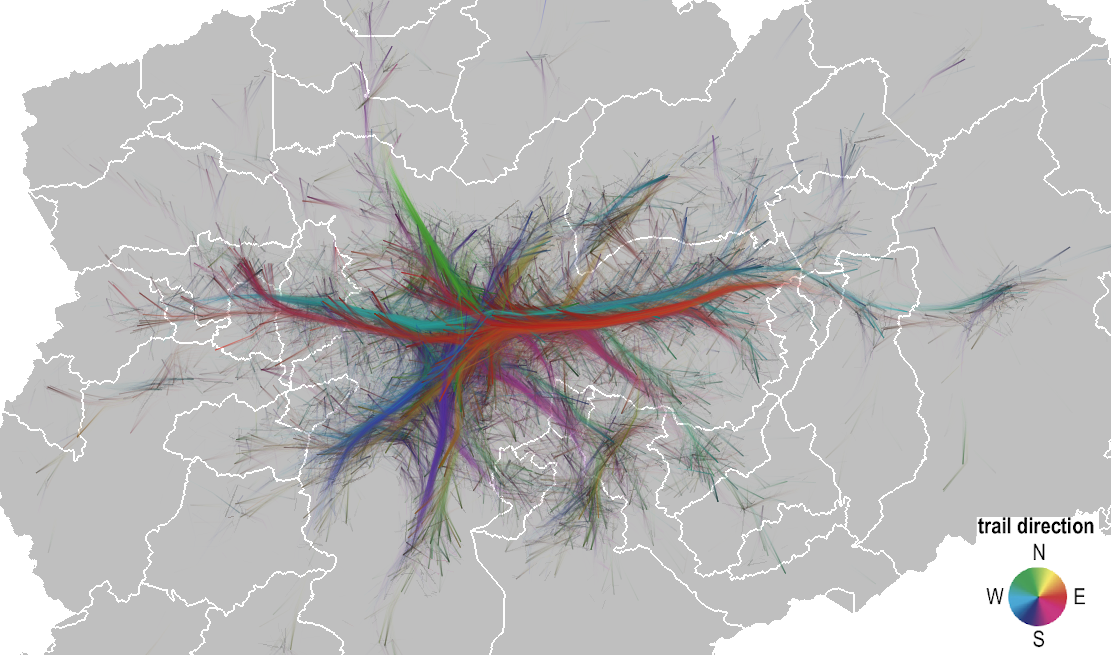
\includegraphics[width=0.98\textwidth]{figures/peak-hours-17h-to-20h-direction-leg.png}
%   \caption{Directions of trips between 5 to 8 PM \label{fig:peak-hours-17h-20h}}
% \end{figure}

% Comparing the peak hours, we can see that morning flows going to the SPMA center (Figure~\ref{fig:peak-hours-6h-9h}, cyan bundle)
% are overall denser and longer than the flows coming from the SPMA center during the afternoon/evening peak (Figure~\ref{fig:peak-hours-17h-20h}, red). This suggests that in the morning people are in a hurry to reach their work, while they are less in a hurry to go back home (or to other destinations like schools or the gym) in the afternoon/evening.

% In Figure~\ref{fig:peak-hours-6h-9h}, we can see that flows in the morning peak going to the capital downtown (cyan bundle coming from the east) are denser than opposite flows (red bundle going to the east). Although flows leaving the capital downtown in the morning are thinner than their opposite ones, they also concentrate a large number of trips, especially to the east and southwest. In Figure~\ref{fig:peak-hours-17h-20h}, the opposite flows seem more equally distributed.

\section{Density by transportation mode}
\label{sec:mode}
% %% on foot, bike, car, metro (sliced, density)
% We next split the OD17 data by transportation mode to compare the flow patterns for four different transportation modes: pedestrians, bicycles, cars, and subway. Figures~\ref{fig:mode-pedestrian}~to~\ref{fig:mode-subway} show the respective visualizations.

% \begin{figure}[!htb]
%   \centering
%   \captionsetup{justification=centering}
%   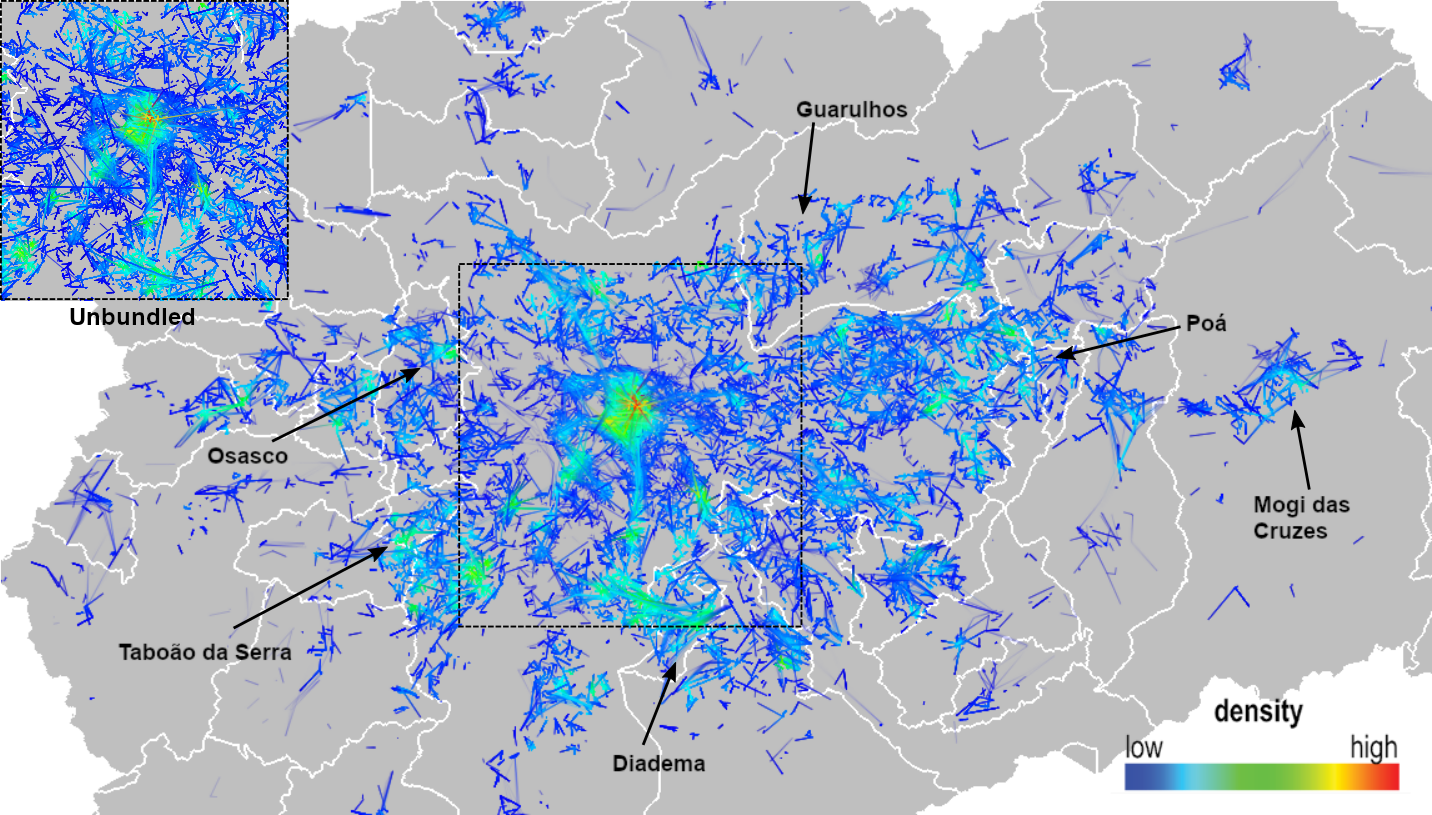
\includegraphics[width=0.98\textwidth]{figures/mode-pedestrian-density-leg.png}
%   \caption{Density of pedestrian trips \label{fig:mode-pedestrian}}
% \end{figure}

% \begin{figure}[!htb]
%   \centering
%   \captionsetup{justification=centering}
%   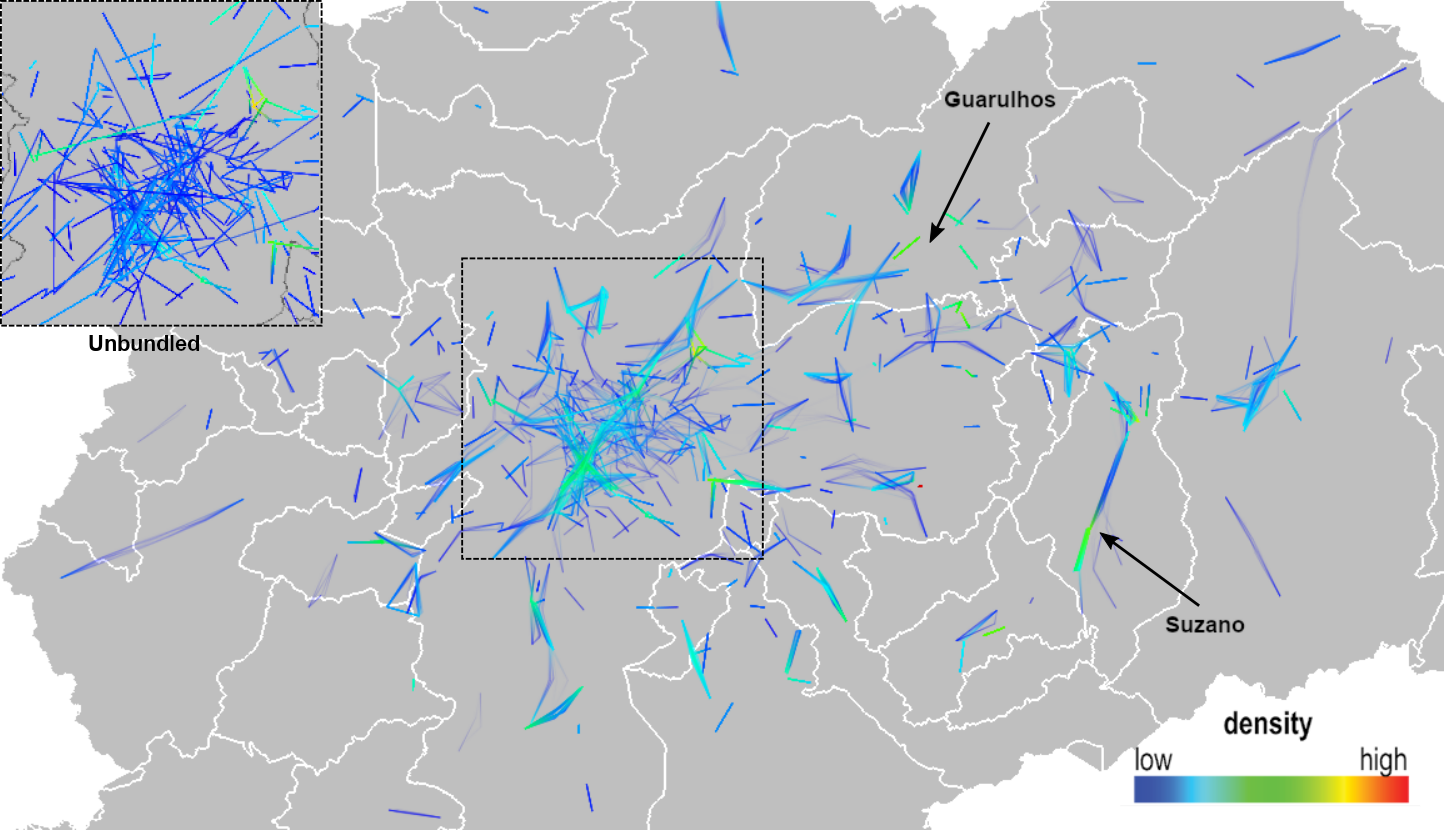
\includegraphics[width=0.98\textwidth]{figures/mode-bike-density-leg.png}
%   \caption{Density of bicycle trips \label{fig:mode-bike}}
% \end{figure}

% \begin{figure}[!htb]
%   \centering
%   \captionsetup{justification=centering}
%   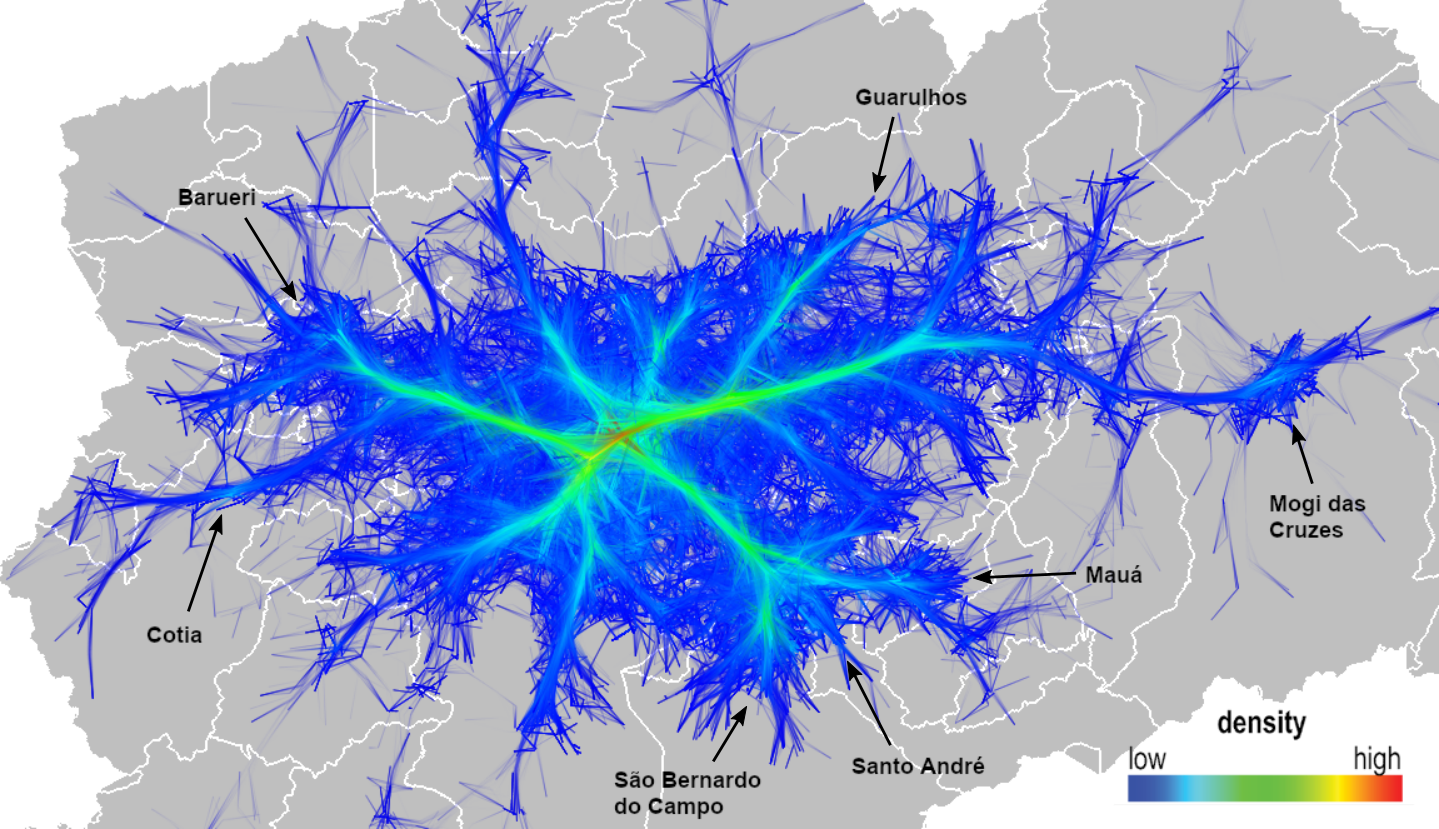
\includegraphics[width=0.98\textwidth]{figures/mode-car-density-leg.png}
%   \caption{Density of car trips \label{fig:mode-car}}
% \end{figure}

% \begin{figure}[!htb]
%   \centering
%   \captionsetup{justification=centering}
%   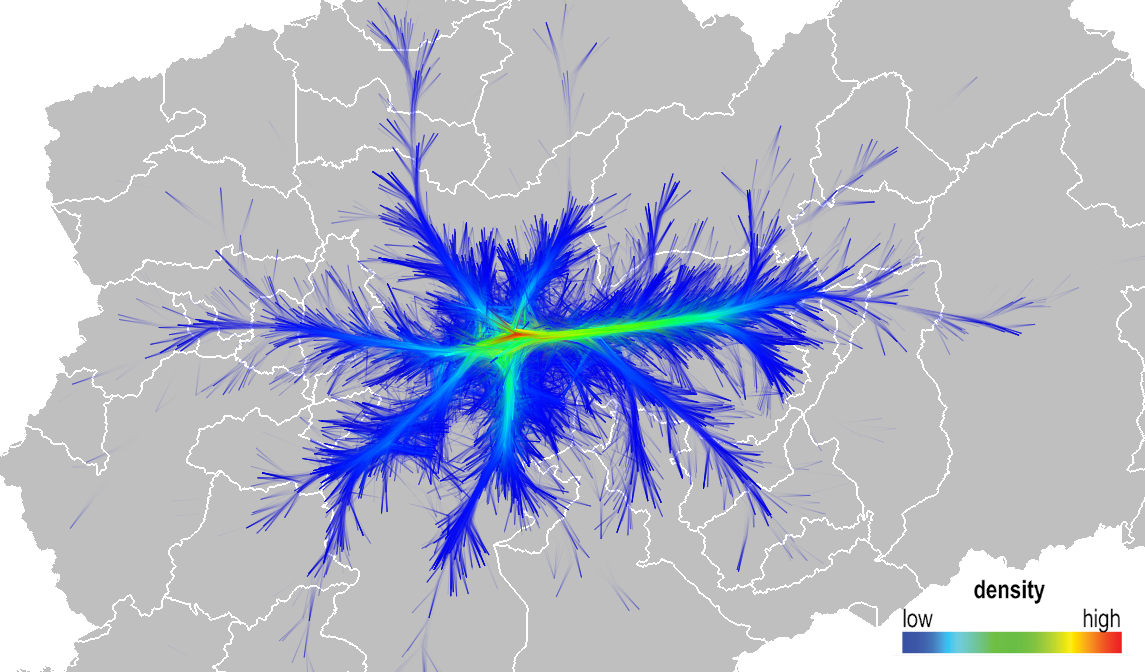
\includegraphics[width=0.98\textwidth]{figures/mode-subway-density-leg.png}
%   \caption{Density of subway trips \label{fig:mode-subway}}
% \end{figure}

% Pedestrian trails (Figure~\ref{fig:mode-pedestrian}) form several low-density `islands' spread across the SPMA, with the densest one (red in figure) being in the capital downtown. Most trails are quite short, which is expected (pedestrians). However, we see a few longer bundles between the capital downtown and the south and north regions of the city. Dense flows are also present in the neighboring cities of Diadema, Tabo\~ao da Serra, Osasco, Guarulhos, Po\'a, and Mogi das Cruzes. Upon examination, we found these dense flows to match the cities' downtown and commercial areas. This information could be useful to find places that could deserve the attention of local governments to provide improvements for pedestrians.

% As most of the pedestrian trips are short, the bundling technique forms a few flows over the SPMA.
% Using bundling for those short trips result in low-density trails, which is less useful compared to long trips. Thus, in these cases it may not be necessary to use bundling. In the upper left area of Figure~\ref{fig:mode-pedestrian}, we can see the OD trails without using bundling, which are near identical to the main bundled area.
% %For pedestrian trails, it would be interesting to apply bundling over small areas. \textbf{AT: Actually, you can do this by running CUBu simply using a much smaller kernel size. But, if we do not do that, I think we should omit the above sentence.}

% Bicycle trips (Figure~\ref{fig:mode-bike}) exhibit similar patterns to pedestrian ones. They are shorter than three kilometers on average. In this figure, we see some thin flows in the capital downtown area. There are also some more salient flows in the capital northeast and in the neighboring cities of Suzano and Guarulhos.
% However, comparing Figure~\ref{fig:mode-bike} with all other transportation means, we immediately see that bicycle trips are by far the least numerous, and exhibit a far sparser pattern, with few star-shaped `hubs' where many trails meet. This suggests that the cycling infrastructure is quite limited, and fragmented. Figure~\ref{fig:mode-bike} also shows trails without using bundling in the upper left corner.

% The car trips (Figure~\ref{fig:mode-car}) show a pattern similar to the one displaying the entire dataset, \emph{i.e.}, all transportation modes (see \emph{e.g.} Figure~\ref{fig:bundled-graph-density}). For a start, this tells that cars are \emph{the} dominant form of transportation in the SPMA, accounting for the main traffic patterns. The highest-density flows occur in the capital downtown. There are several high-density flows linking the downtown area to the other regions of the capital, and also coming and going from the cities of Guarulhos, Barueri, Cotia, S\~ao Bernardo do Campo, Santo Andr\'e, Mau\'a, and Mogi das Cruzes. Compared to all other transportation modes, cars show a far more `spread out' pattern that covers very large areas, indicating that cars are the prevalent transportation mode in most parts of the SPMA.

% Finally, subway trips (Figure~\ref{fig:mode-subway}) show a strong star-shaped pattern, with very high density bundles that connect the capital with the neighboring cities, due to the integration of the subway system with the train system. Compared to all other transportation modes, subways show a clearer, simpler, trip pattern structure.

\section{Different trip reasons}
\label{sec:dist_reasons}
% We next aim to study whether trips done for different reasons exhibit distinct trip patterns. For this, we create bundled visualizations from the OD17 data with trips grouped by work, health, education, and shopping. Figures~\ref{fig:reason-work}~to~\ref{fig:reason-shopping} show the results.

% Work-related trips (Figure~\ref{fig:reason-work}) are overall longer than the other trip reasons, and also cover a larger area (see the central agglomeration in the figure). Interestingly, the longest trips, between the east side and the city center (red bundle), are similar in pattern to the longest trips for health and education. 
% Trips for health reasons are sparser than work-related ones, and also show a more star-like pattern, with long bundles connecting to the central area. This may indicate that peripheral regions are not well served by health services. Trips for studying reasons (Figure~\ref{fig:reason-education}) have the largest distances between the northeast and the western regions of the SPMA. Their pattern is somewhere in-between the work and health trips. Interestingly, education trips show several `loops' in the center of the SPMA. Finally, shopping trips (Figure~\ref{fig:reason-shopping}) show the least dense, and overall also shortest, patterns, apart from a few outliers like the red (important) bundle connecting the center to the northeast. This tells that, unlike health, education, and work, shopping facilities (which are actually provided by private companies) are better distributed over the SPMA. This outlines that bundled visualizations are useful not only when they show the \emph{presence} of certain data, \emph{e.g.} trails linking far-apart regions; the \emph{absence} of patterns is also insightful, as in the case of the lack of long shopping trips.

% \begin{figure}[!htb]
% \centering
% \captionsetup{justification=centering}
% 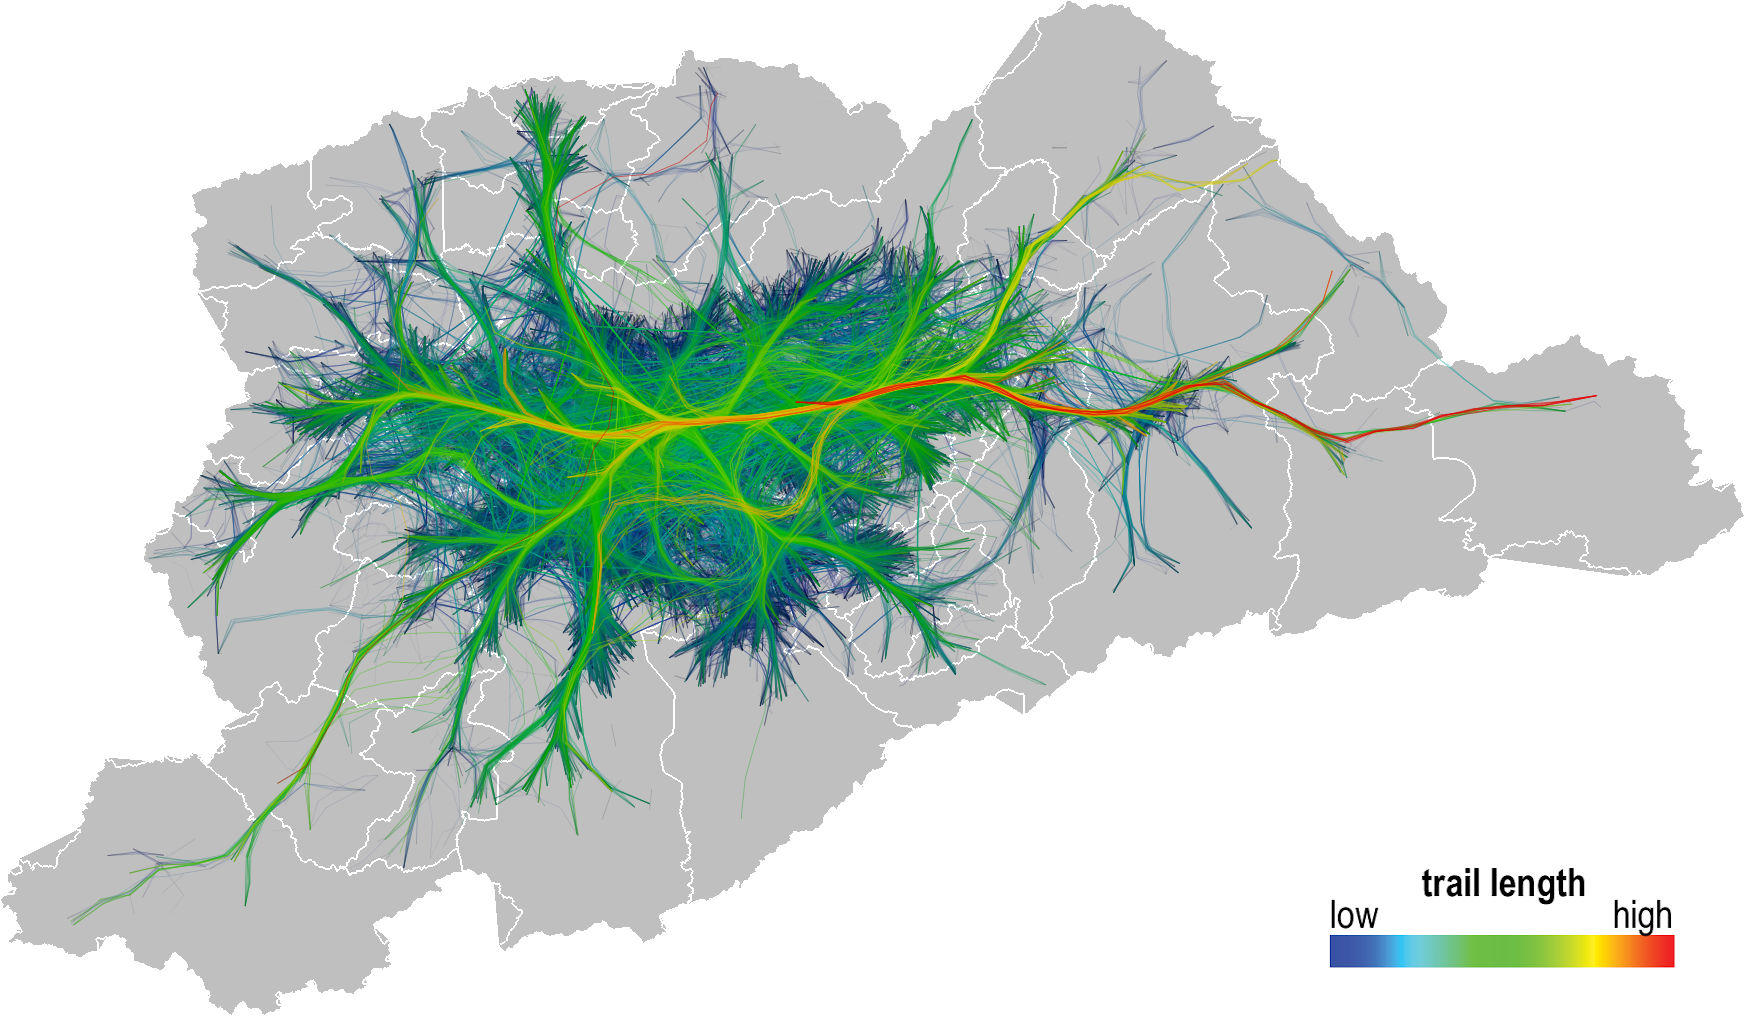
\includegraphics[width=0.98\textwidth]{figures/reason-work-leg.png}
% \caption{Distance of trips for work reasons.\label{fig:reason-work}}
% \end{figure}
  
% \begin{figure}[!htb]
% \centering
% \captionsetup{justification=centering}
% 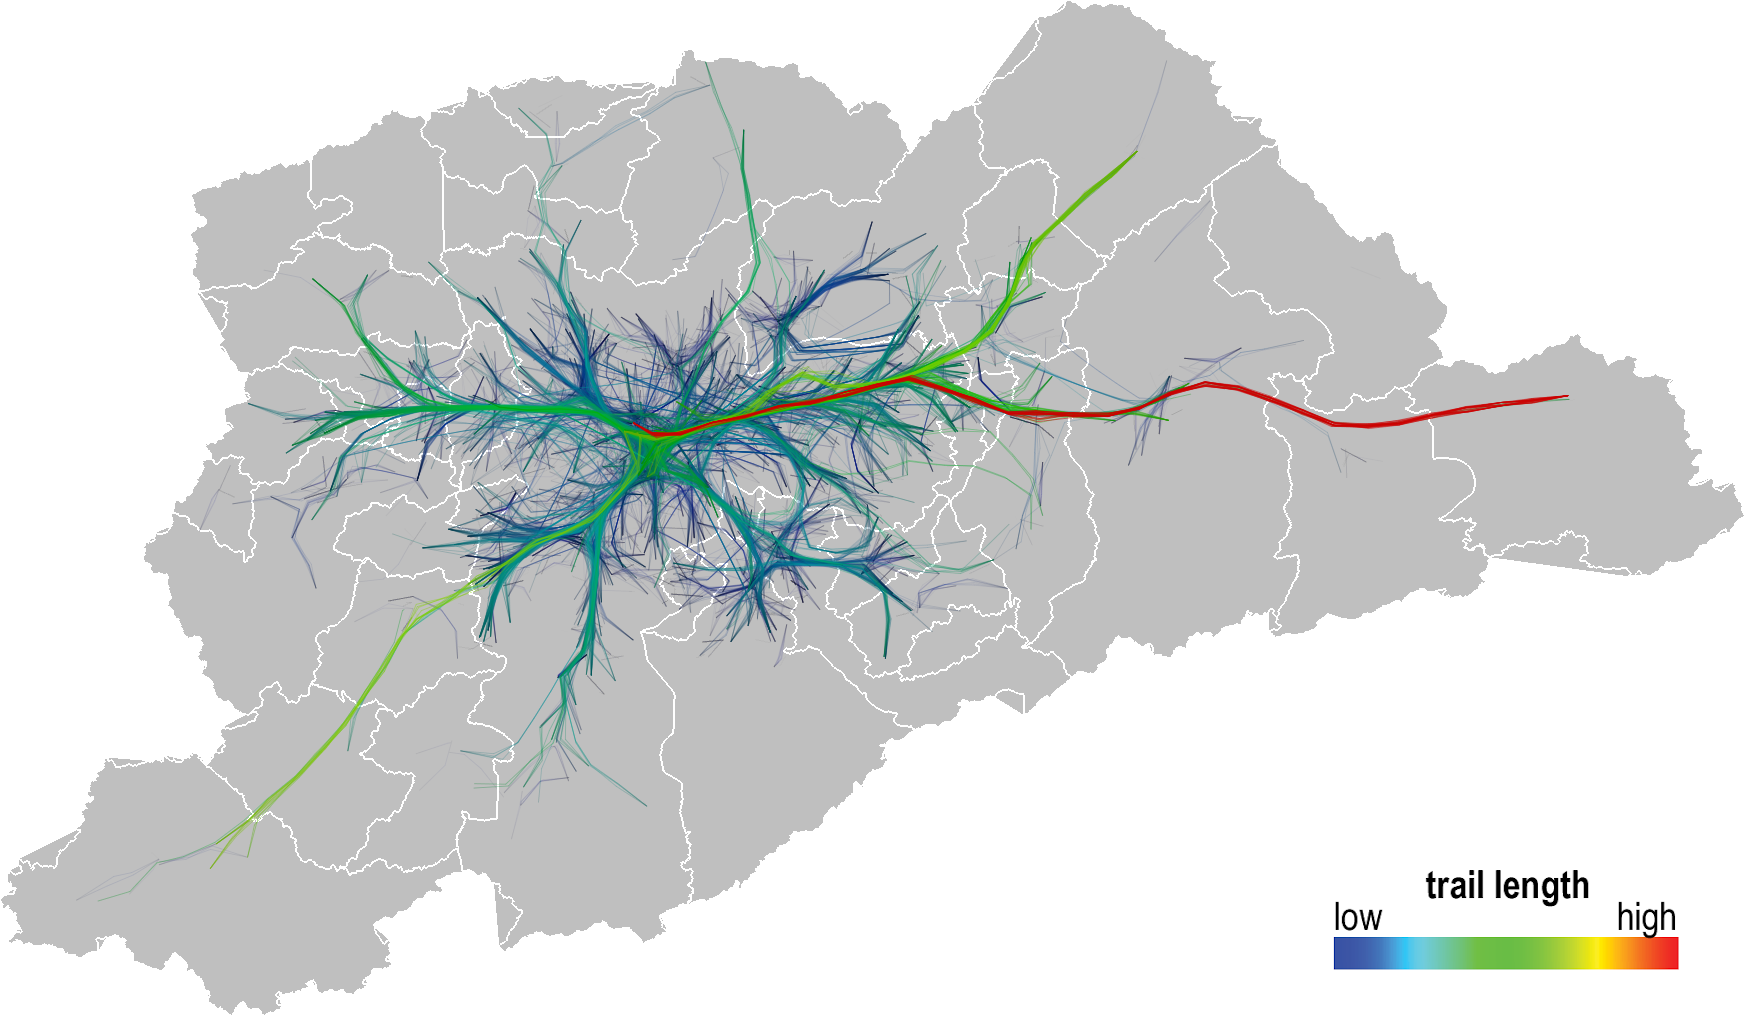
\includegraphics[width=0.98\textwidth]{figures/reason-health-leg.png}
% \caption{Distance of trips for health-related reasons.\label{fig:reason-health}}
% \end{figure}

% \begin{figure}[!htb]
% \centering
% \captionsetup{justification=centering}
% 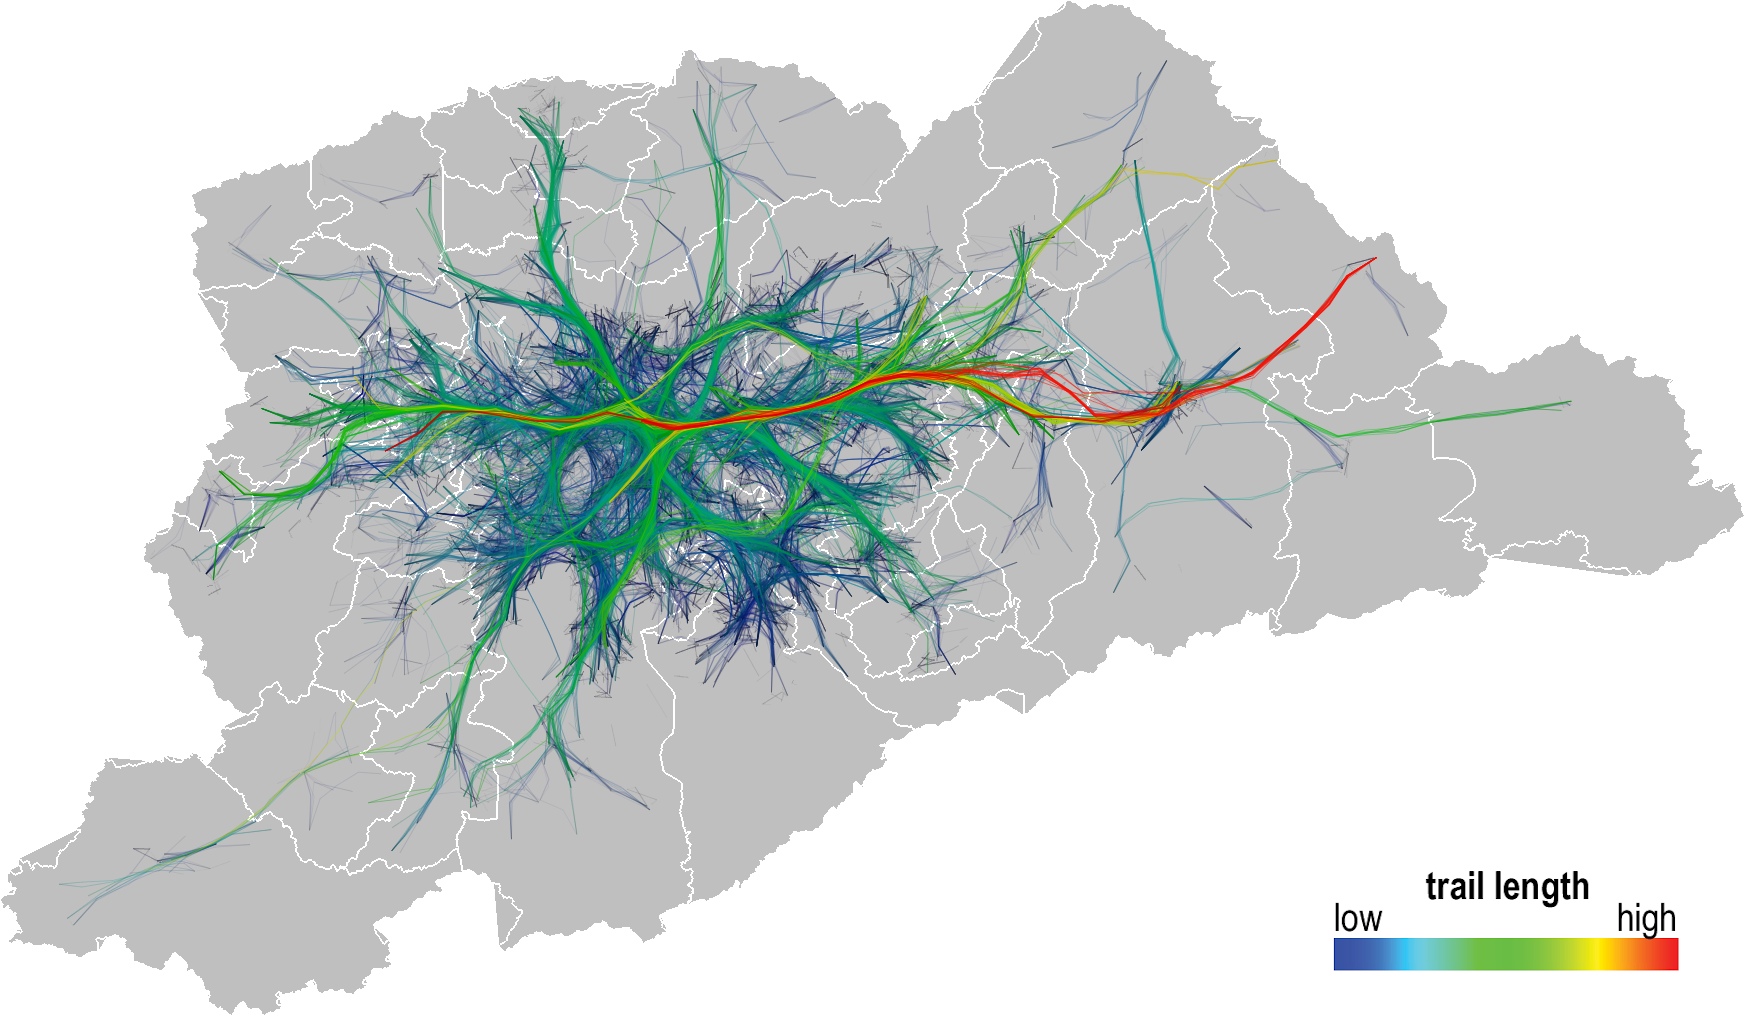
\includegraphics[width=0.98\textwidth]{figures/reason-school-leg.png}
% \caption{Distance of trips for education reasons.\label{fig:reason-education}}
% \end{figure}

% \begin{figure}[!htb]
% \centering
% \captionsetup{justification=centering}
% 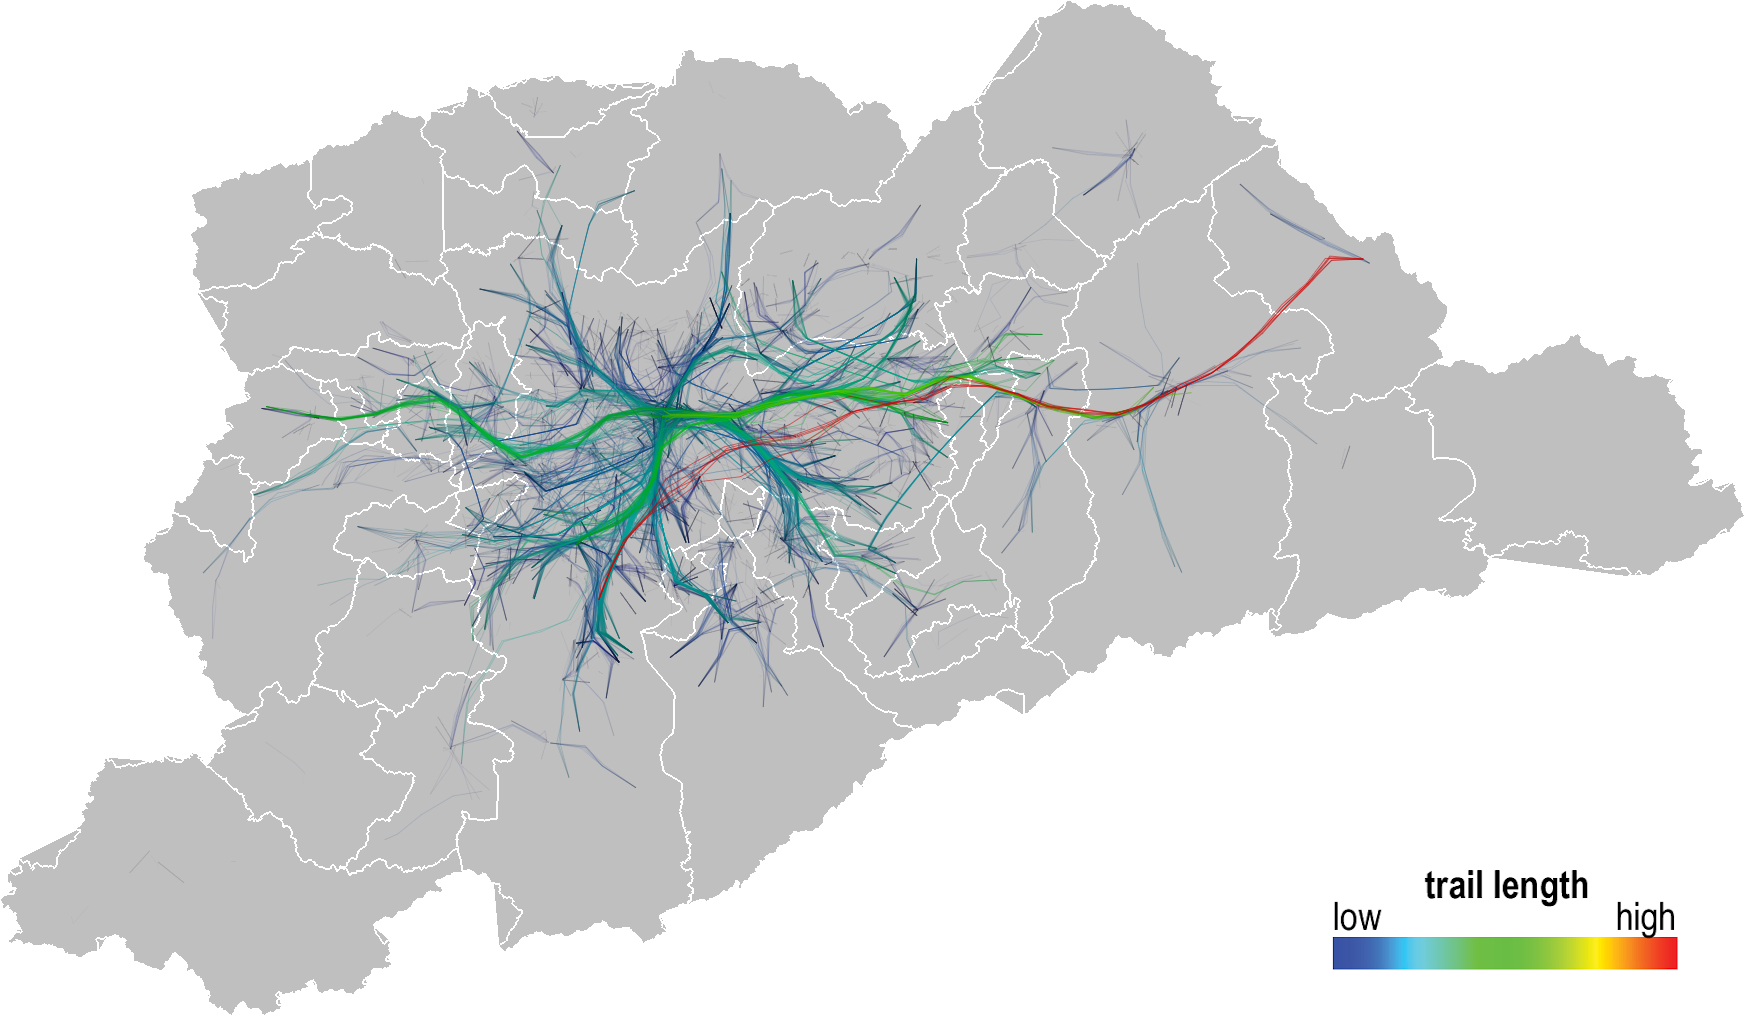
\includegraphics[width=0.98\textwidth]{figures/reason-shopping-leg.png}
% \caption{Distance of trips for shopping reasons.\label{fig:reason-shopping}}
% \end{figure}

